% .s1 manuscript, IEEE/ACM Transactions on Computational Biology and Bioinformatics (IEEEtran, compsoc journal).
% Every result is a macro \nm{key} defined in generated/numbers.tex, and every plotted value is read from generated/*.tsv;
% both are written by `python -m s1bench report` (bench/). A key the pipeline has not produced prints as a red [??key].
% The supplement (supplement.tex) and the format specification (spec.tex) are separate documents; references between
% main and supplement resolve through xr, so build both twice:  latexmk -pdf supplement.tex main.tex  (run it twice).
\documentclass[10pt,journal,compsoc]{IEEEtran}
% Shared by main.tex (IEEEtran, the TCBB submission), supplement.tex and spec.tex: packages that work under both
% IEEEtran and article, the generated-number macros, house colours and pgfplots settings.
\usepackage[T1]{fontenc}
\usepackage{amsmath,amssymb}
\usepackage[scale=0.9]{plex-sans}   % figure text in IBM Plex, the singlet.bio typefaces
\usepackage[scale=0.86]{plex-mono}
\usepackage{microtype}
\usepackage{booktabs,tabularx,array}
\usepackage{xcolor}
\usepackage{graphicx}
\usepackage{adjustbox}
\usepackage{tikz}
\usetikzlibrary{arrows.meta,positioning,fit,calc,decorations.pathreplacing,backgrounds}
\usepackage{pgfplots}
\usepackage{pgfplotstable}
\pgfplotsset{compat=1.18}
\usepgfplotslibrary{fillbetween}

% ---------- generated numbers ----------
\newcommand{\defnum}[2]{\expandafter\def\csname s1n@#1\endcsname{#2}}
\newcommand{\nm}[1]{\ifcsname s1n@#1\endcsname\csname s1n@#1\endcsname\else\textcolor{red!75!black}{\text{\sffamily\footnotesize[??\detokenize{#1}]}}\fi}
\InputIfFileExists{generated/numbers.tex}{}{}
\newcommand{\gen}[1]{generated/#1}   % path of a generated table

% ---------- house style ----------
\newcommand{\sone}{\texttt{.s1}}
% singlet.bio brand (singlet.bio/brand): teal for .s1, ink and grey-green neutrals, violet and amber accents
\definecolor{sone}{HTML}{0E8C7E}   % teal 500
\definecolor{gen}{HTML}{6B7C78}    % neutral, between muted and cell
\definecolor{dom}{HTML}{C2410C}
\definecolor{dl}{HTML}{B42318}     % limits: the floor of the count models
\definecolor{dec}{HTML}{B45309}    % amber: entropy coders, the output bound
\definecolor{tens}{HTML}{7C5CFF}   % violet: fitted trends
\definecolor{ink2}{HTML}{2B3F3C}   % ink 2
% .s1 in singlet.bio teal and every other format in one gray, in every panel that shows formats; labels name them.
% Color names are c-<format id>, the ids of the `format` column of generated/*.tsv.
\definecolor{c-s1}{HTML}{0E8C7E}
\definecolor{c-h5ad_none}{HTML}{9BA3A1}
\definecolor{c-h5ad_lzf}{HTML}{9BA3A1}
\definecolor{c-h5ad_gzip}{HTML}{9BA3A1}
\definecolor{c-tenx_h5}{HTML}{9BA3A1}
\definecolor{c-loom}{HTML}{9BA3A1}
\definecolor{c-zarr}{HTML}{9BA3A1}
\definecolor{c-zarr3}{HTML}{9BA3A1}
\definecolor{c-soma}{HTML}{9BA3A1}
\definecolor{c-bpcells}{HTML}{9BA3A1}
\definecolor{c-parquet_coo}{HTML}{9BA3A1}
\definecolor{c-mtx_gz}{HTML}{9BA3A1}
\definecolor{c-csc_i32}{HTML}{9BA3A1}
\definecolor{c-csc_zstd19}{HTML}{9BA3A1}
\definecolor{c-rds_gz}{HTML}{9BA3A1}
\definecolor{c-rds_xz}{HTML}{9BA3A1}
% every format but .s1, for loops over plots
\def\otherformats{h5ad_none,h5ad_lzf,h5ad_gzip,tenx_h5,loom,zarr,zarr3,soma,bpcells,parquet_coo,mtx_gz,csc_i32,csc_zstd19,rds_gz,rds_xz}

\emergencystretch=3em
\renewcommand{\topfraction}{0.95}\renewcommand{\textfraction}{0.05}\renewcommand{\floatpagefraction}{0.7}
\renewcommand{\dbltopfraction}{0.95}\renewcommand{\dblfloatpagefraction}{0.7}

% pgfplots: read tab-separated tables; keep only rows whose column #1 equals #2 (x or y filter)
\pgfplotsset{
  table/col sep=tab,
  discard if not/.style 2 args={x filter/.append code={\edef\tempa{\thisrow{#1}}\edef\tempb{#2}\ifx\tempa\tempb\else\def\pgfmathresult{nan}\fi}},
  discard if not y/.style 2 args={y filter/.append code={\edef\tempa{\thisrow{#1}}\edef\tempb{#2}\ifx\tempa\tempb\else\def\pgfmathresult{nan}\fi}},
  every axis/.append style={font=\sffamily\scriptsize, label style={font=\sffamily\scriptsize},
    axis line style={ink2!85}, every tick/.style={ink2!85},
    /pgf/number format/assume math mode=true,   % numbers in the figure font, not math digits
    tick label style={font=\sffamily\tiny}, title style={font=\sffamily\small\bfseries, align=left}},
}
\pgfplotstableset{col sep=tab, empty cells with={--}, every head row/.style={before row=\toprule, after row=\midrule},
  every last row/.style={after row=\bottomrule}}

\newcommand{\placeholder}[1]{\textcolor{red!75!black}{[#1]}}   % text still to be supplied by the author

\usepackage[nocompress]{cite}
\usepackage{xr-hyper}
\usepackage[colorlinks=true,linkcolor=blue!50!black,citecolor=blue!50!black,urlcolor=blue!50!black]{hyperref}
\newcommand{\para}[1]{\par\smallskip\noindent\textbf{#1.}\ }   % run-in paragraph heading
\externaldocument[S-]{supplement}   % supplement labels as S-<label>, so its citation keys do not clash with ours

\begin{document}
\title{Fewer Bits, Faster Cells: An AI-Ready Single-Cell Count Format Near the Limits of Size and Speed}
\author{Zachary~J.~DeBruine%
\IEEEcompsocitemizethanks{\IEEEcompsocthanksitem Z.\,J.~DeBruine is with the Department of Information Sciences and
Technology, College of Computing, Grand Valley State University, Allendale, MI, USA.\protect\\
E-mail: debruinz@gvsu.edu}}

\markboth{IEEE/ACM Transactions on Computational Biology and Bioinformatics}%
{DeBruine: Fewer Bits, Faster Cells}

\IEEEtitleabstractindextext{%
\begin{abstract}
% Abstract, shared by main.tex (TCBB) and biorxiv.tex. About 250 words.
The Gene Expression Omnibus holds sequencing data from more than three billion cells. Machine learning models now train
on millions of them at a time, streamed from cloud storage in minibatches, and AI agents fetch and analyze public data
themselves, waiting on every fetch as they iterate. Both spend much of their time moving and decoding count matrices,
so alongside systematic annotation, small files that open with low latency are what make data AI-ready. We measured how few bits these
counts need and how fast they can be decoded, then built \sone{} to approach both limits, using Claude 5.5-generation
models (Anthropic). A \sone{} dataset is a manifest of content-addressed sample files, each opening with an index to
blocks of cells, so a reader fetches only the cells it needs by HTTP range request. Within a block, each cell becomes
small steps between genes and small counts, which an rANS coder encodes with tables chosen by the cell's depth, in 32
SIMD lanes. On \nm{nMatrices} public matrices, \sone{} files were the smallest on every one, \nm{ratioBestOther} times
smaller than the best alternative and within a few percent of cross-validated count models; in UMI data most remaining
bits are molecular sampling, irreducible given each cell's expression rates. On four cores \sone{} read fastest on
\nm{dec-s1-fastest-count} of \nm{dec-paired-n} matrices, and from a real cloud object store it delivered a first PyTorch
minibatch in under a second and streamed cells tens of times faster than Zarr, though per core its decoder is slower than
byte-oriented codes. \sone{} brings single-cell count matrices close to the limits of size and speed, ready to be shared
quickly and read in part by models and agents alike.

\end{abstract}

\begin{IEEEkeywords}
Data compression, entropy coding, sparse matrices, single-cell RNA sequencing, file formats, cloud storage, machine
learning data loading.
\end{IEEEkeywords}}

\maketitle
\IEEEdisplaynontitleabstractindextext
\IEEEpeerreviewmaketitle

% Introduction (main text). Numbers belong in the figures and their captions; the text states what they show.
\section{Introduction}
\label{sec:intro}

\IEEEPARstart{H}{ow} many bits does a single cell need? The Gene Expression Omnibus~\cite{barrett2013geo} now holds sequencing data from more than three billion cells~\cite{seqout}, reference atlases serve tens of
millions~\cite{svensson2018exponential,sikkema2023integrated,czi2025cellxgene}, a single perturbation screen has reached a
hundred million~\cite{zhang2025tahoe}, and machine learning models are trained by streaming such collections from cloud
storage, minibatch by minibatch, many times over~\cite{lopez2018deep,theodoris2023transfer,cui2024scgpt}. AI agents,
too, now find, fetch and analyze public data on their own, deciding after each result what to fetch next. Every one of
those minibatches and fetches crosses a network. When it does, the bits each cell takes and the round trips needed to find
it, not the model or the processor, set how fast training runs, what each epoch costs, and whether an agent can answer
within a conversation or must wait minutes for each step. AI-ready data, we argue, is not just a matter of systematic
annotation but also of how quickly a model can get the cells it needs.

Today's formats spend those bits generously. AnnData~\cite{virshup2024anndata}, the 10x Genomics HDF5 file, loom, Zarr and
TileDB-SOMA~\cite{tiledbsoma} store whole-number counts as generic arrays and hand them to compressors such as gzip or
zstd, which see only bytes. Yet count matrices are anything but arbitrary. Most non-zero counts are exactly one; a cell's
sequencing depth sets the expected count of every gene in it; and if genes are numbered from most to least often
detected, the positions of a cell's non-zero entries become a short list of small steps. Properties like these, specific
to the data, are what let CRAM replace gzip for sequencing reads with models of the reads
themselves~\cite{bonfield2022cram}.

A model of the counts can shrink a file, but a smaller file helps only if it can be decoded as fast as the link delivers
it. So we asked two questions together: how few bits can a lossless code spend on single-cell counts, and how fast can a
code that small be decoded? We measured both limits on \nm{nMatrices} public matrices and built \sone, an open format that
approaches them (Fig.~\ref{fig:how}), read and written from Python, R and C++ by the \texttt{singlet} package. We found
that (Fig.~\ref{fig:wow}):
\begin{itemize}
\item \sone{} files were the smallest on every matrix, \nm{ratio-h5ad_gzip} times smaller than gzip-compressed AnnData and
  within a few percent of the best count models we were able to discover;
\item on four cores, \sone{} was also the fastest format to read on \nm{dec-s1-fastest-count} of \nm{dec-paired-n}
  matrices, and no integer code we measured was both as small and faster to decode;
\item from cloud storage, a PyTorch loader received its first \sone{} minibatch in under a second and then kept a
  1\,Gbit/s link busy where chunked formats left it idle.
\end{itemize}
We also report what \sone{} costs: a decoder that is slower per core, a writer that is slower and needs more memory, and
no traversal of the data in place. The codec was developed iteratively with Claude 5.5-generation models (Anthropic),
with every candidate change measured against the limits above.

% Figure 2: how .s1 stores single-cell counts, as four panels joined by zoom wedges, lettered as sections/format.tex
% cites them: (a) a dataset, (b) one sample file (header, member table, shared packs), (c) one count-matrix member
% (prefix, chunks, range requests), (d) one chunk. Plain words stand in for spec terms: "table of contents" is the
% member table, "block" a chunk, "code tables" the entropy tables, "gene order" the row keys, "symbol" the gap symbol
% (sigma, amber: the residual rho), "coders" the rANS lanes. Sizes, the prefix, the request pattern, the 12 x 40
% contexts (ctx_kind 0) and the chunk byte order follow sections/supplement_spec.tex. Genes, counts and ranks in (d)
% are a worked example of those rules, not data. Request labels in (c) follow the reference client
% (python/singlet/s1/client.py: the first request carries the prefix, then one request per run of chunks).
\begin{figure*}[tbp]
\centering
% panel title with a hanging indent after the panel letter
\def\ptitle#1#2#3#4{\node[ptit, text width=#3] at (#1) {\hyphenpenalty=10000\exhyphenpenalty=10000\hangindent=0.36cm\hangafter=1\makebox[0.36cm][l]{\small #2}#4};}
% station title in panel d
\def\stitle#1#2#3#4{\node[stit, text width=#2] at (#1) {\hyphenpenalty=10000\exhyphenpenalty=10000\hangindent=0.28cm\hangafter=1\makebox[0.28cm][l]{\bfseries #3}#4};}
% zoom wedge from a parent element's corners (#1, #2) to a child panel's corners (#3, #4)
\def\zoomwedge#1#2#3#4{\begin{scope}[on background layer]\fill[sone!5] (#1)--(#3)--(#4)--(#2)--cycle;\draw[wl] (#1)--(#3) (#2)--(#4);\end{scope}}
% one row of the table of contents in (b): y, style, name, start, length
\def\tocrow#1#2#3#4#5{%
  \node[cell,#2,minimum width=1.95cm,anchor=north west] at (7.15,#1) {#3};
  \node[cell,#2,minimum width=0.80cm,anchor=north west,align=center] at (9.10,#1) {#4};
  \node[cell,#2,minimum width=0.80cm,anchor=north west,align=center] at (9.90,#1) {#5};}
% legend chips for the note in (d): blue symbol, amber symbol
\def\chipkey#1#2{{\setlength{\fboxsep}{0pt}\fcolorbox{#1}{#2}{\rule{0pt}{5.5pt}\hspace{8pt}}}}
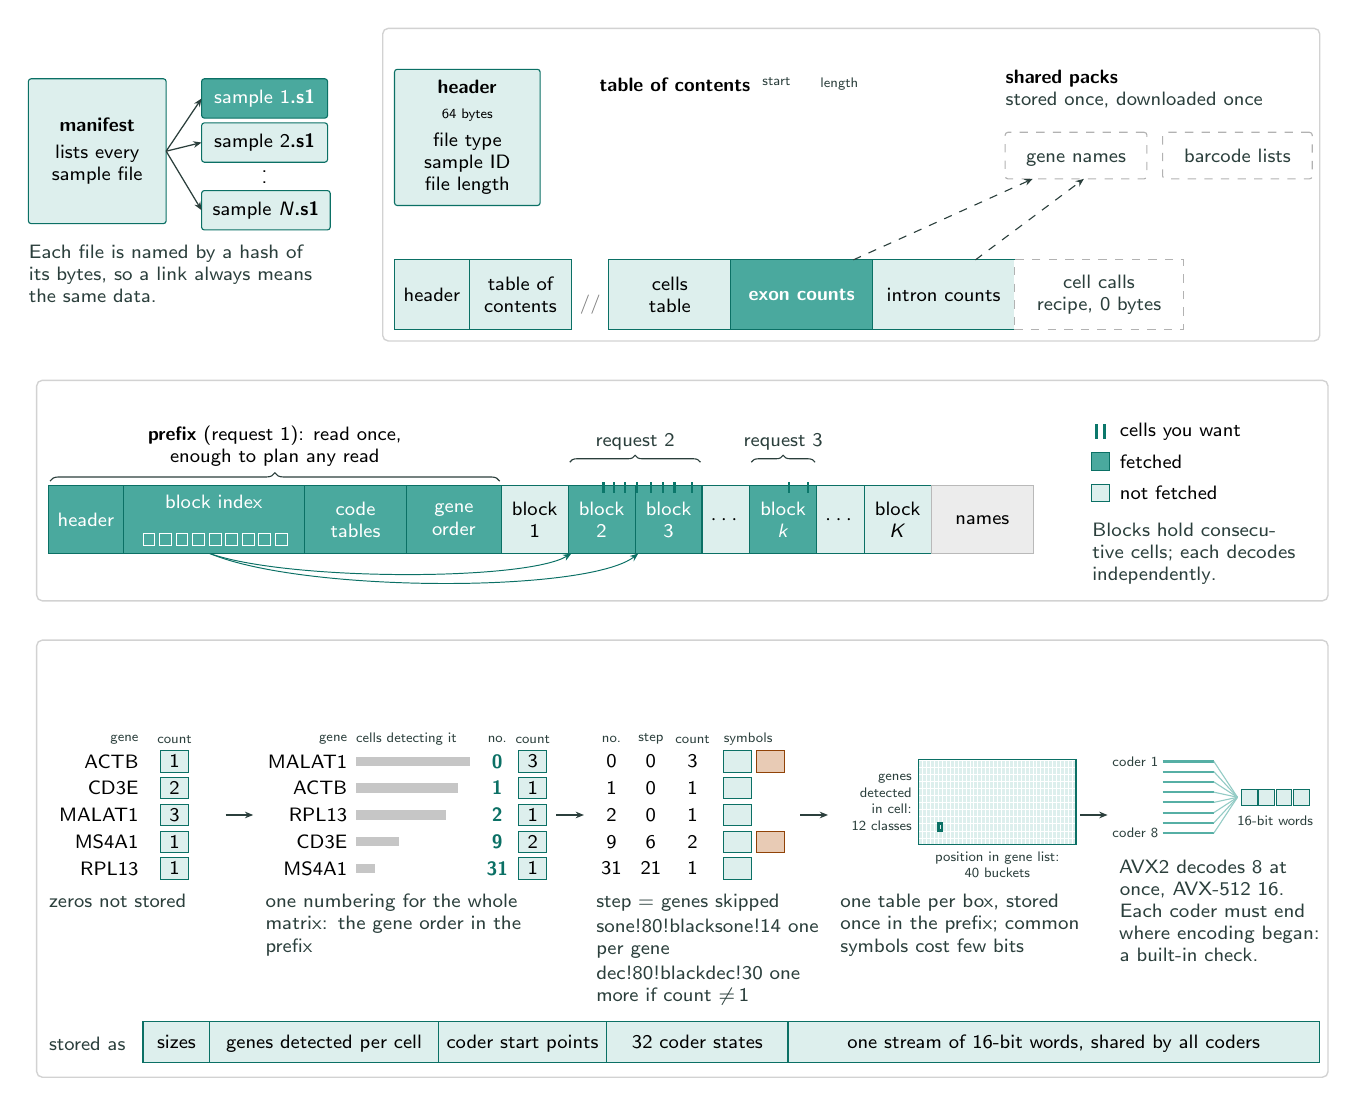
\begin{tikzpicture}[
  x=1cm, y=1cm,
  font=\sffamily\scriptsize,
  >={Stealth[length=3pt,width=2.4pt]},
  st/.style={draw=sone!80!black, fill=sone!14, line width=0.4pt},
  hot/.style={draw=sone!80!black, fill=sone!75, text=white, line width=0.4pt},
  idle/.style={draw=gray!55, fill=gray!15, line width=0.4pt},
  ghost/.style={draw=gray!60, dashed, fill=white, text=ink2, line width=0.4pt},
  amb/.style={draw=dec!80!black, fill=dec!30, line width=0.4pt},
  seg/.style={rectangle, inner sep=3pt, outer sep=0pt, align=center, anchor=south west},
  box/.style={rectangle, inner sep=4pt, outer sep=0pt, align=center, rounded corners=1pt},
  cell/.style={rectangle, inner sep=3pt, outer sep=0pt, align=left, minimum height=0.36cm, text depth=0.5pt},
  frame/.style={draw=gray!35, rounded corners=2pt, line width=0.5pt},
  ptit/.style={font=\sffamily\scriptsize\bfseries, anchor=north west, inner sep=0pt, align=left},
  stit/.style={font=\sffamily\scriptsize, anchor=north west, inner sep=0pt, align=left},
  note/.style={text=ink2, inner sep=0pt, align=left},
  hd/.style={font=\sffamily\tiny, text=ink2, inner sep=0pt},
  wl/.style={draw=gray!55, line width=0.4pt},
  arr/.style={->, ink2, line width=0.45pt},
  chip/.style={rectangle, inner sep=0pt, outer sep=0pt, minimum height=0.27cm, minimum width=0.36cm, line width=0.4pt},
]

% =============================================================== (a) a dataset
\ptitle{0,0}{a}{4.1cm}{A dataset}
\node[box, st, anchor=north west, minimum width=1.75cm, minimum height=1.84cm] (man) at (0,-0.62)
  {\textbf{manifest}\\[2pt]lists every\\sample file};
\node[box, hot, anchor=north west, minimum width=1.6cm, minimum height=0.36cm] (s1) at (2.2,-0.62) {sample 1\textbf{.s1}};
\node[box, st,  anchor=north west, minimum width=1.6cm, minimum height=0.36cm] (s2) at (2.2,-1.18) {sample 2\textbf{.s1}};
\node at (3.0,-1.83) {$\vdots$};
\node[box, st,  anchor=north west, minimum width=1.6cm, minimum height=0.36cm] (sN) at (2.2,-2.04) {sample \textit{N}\textbf{.s1}};
\foreach \s in {s1,s2,sN} \draw[arr] (man.east) -- (\s.west);
\node[note, anchor=north west, text width=3.75cm] at (0,-2.72)
  {Each file is named by a hash of its bytes, so a link always means the same data.};

% =============================================================== (b) one sample file
\draw[frame] (4.5,0.02) rectangle (16.4,-3.95);
\ptitle{4.62,-0.08}{b}{6cm}{One sample file}
% the file as stored
\node[seg, st,  minimum width=0.95cm, minimum height=0.88cm] (hdrB) at (4.65,-3.8) {header};
\node[seg, st,  minimum width=1.30cm, minimum height=0.88cm] (tocB) at (hdrB.south east) {table of\\contents};
\node[seg,      minimum width=0.40cm, minimum height=0.62cm, text=gray] (brkB) at (tocB.south east) {//};
\node[seg, st,  minimum width=1.55cm, minimum height=0.88cm] (celB) at (brkB.south east) {cells\\table};
\node[seg, hot, minimum width=1.80cm, minimum height=0.88cm] (cntB) at (celB.south east) {\textbf{exon counts}};
\node[seg, st,  minimum width=1.80cm, minimum height=0.88cm] (intB) at (cntB.south east) {intron counts};
\node[seg, ghost, minimum width=2.15cm, minimum height=0.88cm] (derB) at (intB.south east) {cell calls\\recipe, 0 bytes};
% zoom: header and table of contents
\node[box, st, anchor=north west, minimum width=1.85cm, minimum height=1.66cm] (hdrZ) at (4.65,-0.5)
  {\textbf{header}\\[1pt]{\tiny 64 bytes}\\[2pt]file type\\sample ID\\file length};
\node[cell, anchor=north west, minimum width=1.95cm, font=\sffamily\scriptsize\bfseries] at (7.15,-0.5) {table of contents};
\node[hd, anchor=north] at (9.50,-0.6) {start};
\node[hd, anchor=north] at (10.30,-0.6) {length};
\tocrow{-0.83}{st}{cells}{\textit{o}\textsubscript{1}}{\textit{l}\textsubscript{1}}
\tocrow{-1.19}{hot}{exon counts}{\textit{o}\textsubscript{2}}{\textit{l}\textsubscript{2}}
\tocrow{-1.55}{st}{intron counts}{\textit{o}\textsubscript{3}}{\textit{l}\textsubscript{3}}
\tocrow{-1.91}{ghost}{cell calls}{0}{0}
\zoomwedge{hdrB.north west}{tocB.north east}{4.65,-2.3}{10.7,-2.3}
% shared packs
\node[note, anchor=north west, text width=3.8cm, text=black] at (12.3,-0.5)
  {\textbf{shared packs}\\\textcolor{ink2}{stored once, downloaded once}};
\node[box, ghost, anchor=north west, minimum width=1.8cm, minimum height=0.5cm, text height=1.6ex, text depth=0.45ex] (pkG) at (12.3,-1.3) {gene names};
\node[box, ghost, anchor=north west, minimum width=1.9cm, minimum height=0.5cm, text height=1.6ex, text depth=0.45ex] (pkB) at (14.3,-1.3) {barcode lists};
\draw[->, dashed, ink2, line width=0.4pt] ($(cntB.north east)+(-0.35,0)$) -- ($(pkG.south west)+(0.35,0)$);
\draw[->, dashed, ink2, line width=0.4pt] ($(intB.north)+(0.3,0)$) -- ($(pkG.south)+(0.1,0)$);

% =============================================================== (c) one count matrix
\begin{scope}[yshift=-0.55cm]
\draw[frame] (0,-3.9) rectangle (16.4,-6.7);
\ptitle{0.12,-4.0}{c}{12cm}{One count matrix: a small prefix, then blocks of cells}
\node[seg, hot, minimum width=0.95cm, minimum height=0.86cm] (hdrC) at (0.15,-6.1) {header};
\node[seg, hot, minimum width=2.30cm, minimum height=0.86cm] (idxC) at (hdrC.south east) {};
\node[text=white, inner sep=0pt] at ($(idxC.north)+(0,-0.2)$) {block index};
\foreach \i in {0,...,8} \draw[white, line width=0.3pt] ($(idxC.south west)+(0.25+0.21*\i,0.1)$) rectangle ++(0.15,0.15);
\node[seg, hot, minimum width=1.30cm, minimum height=0.86cm] (tabC) at (idxC.south east) {code\\tables};
\node[seg, hot, minimum width=1.20cm, minimum height=0.86cm] (ordC) at (tabC.south east) {gene\\order};
\node[seg, st,  minimum width=0.85cm, minimum height=0.86cm] (b1) at (ordC.south east) {block\\1};
\node[seg, hot, minimum width=0.85cm, minimum height=0.86cm] (b2) at (b1.south east) {block\\2};
\node[seg, hot, minimum width=0.85cm, minimum height=0.86cm] (b3) at (b2.south east) {block\\3};
\node[seg, st,  minimum width=0.55cm, minimum height=0.86cm] (bd1) at (b3.south east) {$\cdots$};
\node[seg, hot, minimum width=0.85cm, minimum height=0.86cm] (bk) at (bd1.south east) {block\\\textit{k}};
\node[seg, st,  minimum width=0.55cm, minimum height=0.86cm] (bd2) at (bk.south east) {$\cdots$};
\node[seg, st,  minimum width=0.85cm, minimum height=0.86cm] (bK) at (bd2.south east) {block\\\textit{K}};
\node[seg, idle, minimum width=1.30cm, minimum height=0.86cm] (nmC) at (bK.south east) {names};
% the prefix
\draw[decorate, decoration={brace, amplitude=3pt}, ink2, line width=0.4pt] ($(hdrC.north west)+(0.02,0.06)$) -- ($(ordC.north east)+(-0.02,0.06)$)
  node[midway, above=5pt, note, align=center, text=black] {\textbf{prefix} (request 1): read once,\\enough to plan any read};
% the wanted cells and one request per run of blocks
\foreach \x in {7.20,7.33,7.47,7.62,7.80,7.95,8.10,8.32,9.55,9.80}
  \draw[sone!85!black, line width=0.8pt] (\x,-5.33) -- (\x,-5.19);
\draw[decorate, decoration={brace, amplitude=2.5pt}, ink2, line width=0.4pt] ($(b2.north west)+(0.02,0.3)$) -- ($(b3.north east)+(-0.02,0.3)$)
  node[midway, above=4pt, inner sep=0pt] {request 2};
\draw[decorate, decoration={brace, amplitude=2.5pt}, ink2, line width=0.4pt] ($(bk.north west)+(0.02,0.3)$) -- ($(bk.north east)+(-0.02,0.3)$)
  node[midway, above=4pt, inner sep=0pt] {request 3};
% index entries point at block starts
\draw[->, sone!80!black, line width=0.35pt] (2.2,-6.1) .. controls (3.2,-6.45) and (6.2,-6.45) .. ($(b2.south west)+(0.04,0)$);
\draw[->, sone!80!black, line width=0.35pt] (2.2,-6.1) .. controls (3.4,-6.6) and (7.0,-6.6) .. ($(b3.south west)+(0.04,0)$);
% legend
\draw[sone!85!black, line width=0.9pt] (13.46,-4.64) -- (13.46,-4.46) (13.56,-4.64) -- (13.56,-4.46);
\node[anchor=west, inner sep=0pt] at (13.75,-4.55) {cells you want};
\draw[hot] (13.4,-5.04) rectangle ++(0.22,0.22);
\node[anchor=west, inner sep=0pt] at (13.75,-4.93) {fetched};
\draw[st] (13.4,-5.44) rectangle ++(0.22,0.22);
\node[anchor=west, inner sep=0pt] at (13.75,-5.33) {not fetched};
\node[note, anchor=north west, text width=2.9cm] at (13.4,-5.7) {Blocks hold consecutive cells; each decodes \mbox{independently}.};

% =============================================================== (d) inside one block
\draw[frame] (0,-7.2) rectangle (16.4,-12.75);
\ptitle{0.12,-7.3}{d}{16cm}{Inside one block: each cell becomes small numbers, then short codes}
% --- station 1: one cell's counts
\stitle{0.15,-7.72}{2.3cm}{1}{One cell's counts}
\node[hd, anchor=east] at (1.3,-8.46) {gene};
\node[hd] at (1.75,-8.46) {count};
\foreach \g/\v [count=\i from 0] in {ACTB/1,CD3E/2,MALAT1/3,MS4A1/1,RPL13/1} {
  \node[anchor=east, inner sep=0pt] at (1.3,{-8.74-0.34*\i}) {\g};
  \node[chip, st] at (1.75,{-8.74-0.34*\i}) {\v};}
\node[note, anchor=north west] at (0.15,-10.42) {zeros not stored};
\draw[arr] (2.4,-9.42) -- (2.75,-9.42);
% --- station 2: genes numbered by detection
\stitle{2.9,-7.72}{3.6cm}{2}{Genes numbered, most often detected first}
\node[hd, anchor=east] at (3.95,-8.46) {gene};
\node[hd, anchor=west] at (4.05,-8.46) {cells detecting it};
\node[hd] at (5.85,-8.46) {no.};
\node[hd] at (6.3,-8.46) {count};
\foreach \g/\w/\d/\v [count=\i from 0] in {MALAT1/1.45/0/3,ACTB/1.3/1/1,RPL13/1.15/2/1,CD3E/0.55/9/2,MS4A1/0.25/31/1} {
  \node[anchor=east, inner sep=0pt] at (3.95,{-8.74-0.34*\i}) {\g};
  \fill[gray!45] (4.05,{-8.80-0.34*\i}) rectangle ++(\w,0.12);
  \node[font=\sffamily\scriptsize\bfseries, text=sone!80!black, inner sep=0pt] at (5.85,{-8.74-0.34*\i}) {\d};
  \node[chip, st] at (6.3,{-8.74-0.34*\i}) {\v};}
\node[note, anchor=north west, text width=3.6cm] at (2.9,-10.42) {one numbering for the whole matrix: the gene order in the prefix};
\draw[arr] (6.6,-9.42) -- (6.95,-9.42);
% --- station 3: steps and counts become symbols
\stitle{7.1,-7.72}{3.0cm}{3}{Small steps and small counts}
\node[hd] at (7.3,-8.46) {no.};
\node[hd] at (7.8,-8.46) {step};
\node[hd] at (8.33,-8.46) {count};
\node[hd, anchor=west] at (8.72,-8.46) {symbols};
\foreach \d/\s/\v/\two [count=\i from 0] in {0/0/3/1,1/0/1/0,2/0/1/0,9/6/2/1,31/21/1/0} {
  \node[inner sep=0pt] at (7.3,{-8.74-0.34*\i}) {\d};
  \node[inner sep=0pt] at (7.8,{-8.74-0.34*\i}) {\s};
  \node[inner sep=0pt] at (8.33,{-8.74-0.34*\i}) {\v};
  \node[chip, st, anchor=west] at (8.72,{-8.74-0.34*\i}) {};
  \ifnum\two=1 \node[chip, amb, anchor=west] at (9.14,{-8.74-0.34*\i}) {};\fi}
\node[note, anchor=north west, text width=3.0cm] at (7.1,-10.42)
  {step = genes skipped\\[1pt]
   \chipkey{sone!80!black}{sone!14}\ one per gene\\[1pt]
   \chipkey{dec!80!black}{dec!30}\ one more if count $\neq$\,1};
\draw[arr] (9.7,-9.42) -- (10.05,-9.42);
% --- station 4: a code table chosen by context
\stitle{10.2,-7.72}{3.0cm}{4}{Short codes for common symbols}
\begin{scope}[shift={(11.2,-9.8)}]
  \fill[sone!14] (0,0) rectangle (2.0,1.08);
  \draw[white, line width=0.15pt, xstep=0.05, ystep=0.09] (0,0) grid (2.0,1.08);
  \draw[sone!80!black, line width=0.4pt] (0,0) rectangle (2.0,1.08);
  \draw[sone!80!black, line width=0.9pt] (5*0.05,2*0.09) rectangle ++(0.05,0.09);
\end{scope}
\node[hd, align=right, anchor=east] at (11.12,-9.26) {genes\\detected\\in cell:\\12 classes};
\node[hd, anchor=north, align=center] at (12.2,-9.88) {position in gene list:\\40 buckets};
\node[note, anchor=north west, text width=3.1cm] at (10.2,-10.42)
  {one table per box, stored once in the prefix; common symbols cost few bits};
\draw[arr] (13.25,-9.42) -- (13.6,-9.42);
% --- station 5: 32 coders, one word stream
\stitle{13.75,-7.72}{2.55cm}{5}{32 rANS coders side by side (8 shown)}
\foreach \l in {0,...,7} {
  \draw[sone!70, line width=0.8pt] (14.3,{-8.74-0.13*\l}) -- (14.95,{-8.74-0.13*\l});
  \draw[sone!45, line width=0.4pt] (14.95,{-8.74-0.13*\l}) -- (15.25,-9.195);}
\node[hd, anchor=east] at (14.25,-8.74) {coder 1};
\node[hd, anchor=east] at (14.25,-9.65) {coder 8};
\foreach \w in {0,...,3} \draw[st] (15.3+0.22*\w,-9.295) rectangle ++(0.2,0.2);
\node[hd, anchor=north] at (15.73,-9.42) {16-bit words};
\node[note, anchor=north west, text width=2.55cm] at (13.75,-9.98)
  {AVX2 decodes 8 at once, AVX-512 16. Each coder must end where encoding began: a \mbox{built-in} check.};
% --- the block as stored
\node[anchor=west, inner sep=0pt, text=ink2] at (0.15,-12.33) {stored as};
\node[seg, st, minimum width=0.85cm, minimum height=0.46cm, text height=1.6ex, text depth=0.45ex] (f1) at (1.35,-12.56) {sizes};
\node[seg, st, minimum width=2.9cm, minimum height=0.46cm, text height=1.6ex, text depth=0.45ex] (f2) at (f1.south east) {genes detected per cell};
\node[seg, st, minimum width=2.1cm, minimum height=0.46cm, text height=1.6ex, text depth=0.45ex] (f3) at (f2.south east) {coder start points};
\node[seg, st, minimum width=2.3cm, minimum height=0.46cm, text height=1.6ex, text depth=0.45ex] (f4) at (f3.south east) {32 coder states};
\node[seg, st, minimum width=6.75cm, minimum height=0.46cm, text height=1.6ex, text depth=0.45ex] (f5) at (f4.south east) {one stream of 16-bit words, shared by all coders};

\end{scope}
% =============================================================== zoom wedges
\zoomwedge{cntB.south west}{cntB.south east}{0,-4.45}{16.4,-4.45}
\zoomwedge{bk.south west}{bk.south east}{0,-7.75}{16.4,-7.75}
\zoomwedge{s1.north east}{s1.south east}{4.5,0.02}{4.5,-3.95}
\end{tikzpicture}
\caption{\textbf{How \sone{} stores single-cell counts.}
\textbf{(a)} A dataset lists per-sample files, each named by a hash of its bytes.
\textbf{(b)} A header and table of contents locate each part; gene names and barcodes sit in shared packs, and
derivable tables are recipes verified on that sample.
\textbf{(c)} A small prefix plans any read, so a reader fetches only the blocks (chunks) of cells it needs.
\textbf{(d)} Genes numbered by detection turn each cell into small steps and counts, coded in few bits with tables
chosen by context.}
\label{fig:how}
\end{figure*}


% Related work (main text): prior work only; results of this paper are in results.tex.
\section{Related work}
\label{sec:related}

\para{Storing count matrices}On disk, almost every single-cell toolkit stores the compressed sparse column (CSC) layout of
its in-memory matrices~\cite{bates2024matrix,virtanen2020scipy}: 32-bit row indices and 32- or 64-bit values, 64 to 96
bits per non-zero, however small the counts are. Matrix Market~\cite{boisvert1997matrix} writes them as text; the 10x HDF5
file~\cite{zheng2017massively,tenx_h5}, loom~\cite{loompy} and AnnData~\cite{virshup2024anndata} (in HDF5~\cite{hdf5} or
Zarr~\cite{zarr}) store chunked arrays, compressed by byte-level filters such as gzip, LZF, Blosc or
zstd~\cite{deutsch1996deflate,collet2021zstd}. Formats built for scale add structure: TileDB-SOMA~\cite{papadopoulos2016tiledb,tiledbsoma}
serves the CELLxGENE Census~\cite{czi2025cellxgene}, BPCells~\cite{parks2025bpcells} bit-packs deltas and values for
streaming reads, and Parquet~\cite{parquet} distributes the largest training corpora~\cite{tahoe100m_hf}. Our earlier VCSC
and IVCSC layouts store each distinct value of a column once and delta-encode and byte-pack its row indices, shrinking
single-cell matrices several-fold below CSC in memory~\cite{ruiter2024vcsc,wolfgang2024vcsc}. None of these uses an entropy coder with a
model of the counts.

\para{Compressing integers}Inverted indexes face the same problem as CSC row indices: sorted integer lists with small gaps.
Byte- and bit-aligned codes~\cite{lemire2018stream,lemire2015decoding} decode billions of integers per second because they
ignore the distribution of the values; entropy coders spend close to $-\log_2 p$ bits per symbol~\cite{cover2006elements}
at a higher cost per symbol. Asymmetric numeral systems~\cite{duda2013asymmetric} with interleaved states decode several
symbols at once on SIMD units~\cite{giesen2014interleaved}, and ANS with contexts closes much of the gap between fast and
small codes for inverted indexes~\cite{moffat2017ans,moffat2020large,pibiri2021techniques}, the closest precedent for
\sone.

\para{Models of genomic data}CRAM~3.1 replaced BAM's gzip blocks with per-field models and 32-way interleaved
rANS~\cite{bonfield2022cram}; benchmarks of read compressors found that how each field is modeled matters more than the
back-end coder~\cite{numanagic2016comparison,hernaez2019genomic}, and genotype matrices have compressors of their
own~\cite{danek2018gtc,lan2021genozip}. For counts, UMI data are close to Poisson samples of a cell's molecules given its
depth~\cite{townes2019feature,kim2020demystifying}, with a negative binomial for biological
variation~\cite{svensson2020droplet,hafemeister2019normalization} and heavy-tailed expression across
genes~\cite{furusawa2003zipf}. These models say what a coder can exploit, and which bits no lossless code can remove.

\para{Feeding models}Training draws random minibatches of cells many times over. scDataset fetches blocks of contiguous
cells and shuffles them in a buffer~\cite{dascenzo2025scdataset}, the Census provides a loader over
TileDB-SOMA~\cite{tiledbsomaml}, and cloud-native formats such as Zarr cut round trips, each of which waits tens of
milliseconds, with independently addressable chunks~\cite{abernathey2021cloud,durner2023exploiting}. These loaders
optimize access over existing encodings; \sone{} changes the encoding.

% The .s1 format (main text). The normative specification is a separate supplementary file (spec.tex).
\section{The \sone{} format}
\label{sec:format}\label{sec:how}

Fig.~\ref{fig:how} shows the format from a whole dataset down to individual bits; the full specification is a separate
supplementary file. A dataset is a small manifest that lists one file per sample, each named by a cryptographic hash of
its contents, so a link always refers to exactly the same bytes and anyone can check them (Fig.~\ref{fig:how}a).
Information shared by many samples, such as the gene names of a genome annotation, is stored once and downloaded once
(Fig.~\ref{fig:how}b). Table~\ref{tab:props} compares these properties with those of other formats.

\para{Blocks for partial reads}How does a reader get a few hundred cells out of a remote file without reading the rest?
Each count matrix starts with a small index that says where every block of consecutive cells lives in the file, and each
block decodes on its own (Fig.~\ref{fig:how}c). A reader fetches the index once and then only the blocks it needs, with one
request per run of blocks, from a local disk, a web server or a cloud bucket alike. Because every block is located before
any is read, all the requests of a minibatch can be sent at once.

\para{A model of the counts}Inside a block, genes are numbered from most to least frequently detected, so each cell's
non-zero entries become a sequence of small steps and small counts, most of them ones. Each entry becomes one short
symbol, and its probability is looked up in a table chosen by two things the reader already knows: how many entries the
cell has, and how far along the gene list it is (Fig.~\ref{fig:how}d). An rANS entropy coder~\cite{duda2013asymmetric}
then spends close to the minimum number of bits on each symbol. The tables are fixed for the whole matrix, so decoding is
a few table look-ups per entry, and 32 coders run side by side so that a processor with AVX2 decodes eight to sixteen
symbols at once. Writing a file ends with a full decode that must reproduce the input exactly.

% Figure 1: the headline. (a) a schematic of what .s1 does differently; (b-g) every value read from generated/*.tsv and
% generated/*_boxes.tex (written by `python -m s1bench report`). One tikzpicture with the axes on a grid: b and c share
% their rows (one per format), d is square, e and f share their rows (one per loader) under b and c, g sits under d.
% \figbox{pos}{q1}{median}{q3}{low whisker}{high whisker}{colour}: one horizontal box, in axis coordinates.
\newcommand{\figbox}[7]{%
  \draw[#7!80!black, line width=0.5pt] (axis cs:#5,#1) -- (axis cs:#2,#1);
  \draw[#7!80!black, line width=0.5pt] (axis cs:#4,#1) -- (axis cs:#6,#1);
  \draw[#7!80!black, fill=#7, fill opacity=0.18, line width=0.5pt] (axis cs:#2,{#1-0.32}) rectangle (axis cs:#4,{#1+0.32});
  \draw[#7!70!black, line width=1.2pt] (axis cs:#3,{#1-0.32}) -- (axis cs:#3,{#1+0.32});}
\begin{figure*}[tbp]
\centering
\pgfmathsetlengthmacro{\figT}{max(\linewidth,18.1cm)}   % design width: panel a needs 18.1 cm; scaled to fit below
\pgfmathsetlengthmacro{\figY}{2.15cm}             % y tick labels of b and e
\pgfmathsetlengthmacro{\figGap}{0.9cm}            % between b and c, e and f (shared rows)
\pgfmathsetlengthmacro{\figD}{4.9cm}              % side of the square panel d (as placed by report_r3.FIG1D_SIDE)
\pgfmathsetlengthmacro{\figDG}{1.5cm}             % before d and g: their y labels
\pgfmathsetlengthmacro{\figW}{(\figT-\figY-\figGap-\figDG-\figD-0.25cm)/2}   % width of b, c, e and f: rows fill \figT
\ifdefined\IEEEtransversionmajor                  % TCBB: the figure and caption fill a page
  \pgfmathsetlengthmacro{\figH}{4.2cm}            % height of e, f and g
  \pgfmathsetlengthmacro{\figV}{2.0cm}            % between rows: x labels below, titles above
  \pgfmathsetlengthmacro{\figA}{5.6cm}            % top of the figure to the top of b and c
\else
  \pgfmathsetlengthmacro{\figH}{3.0cm}
  \pgfmathsetlengthmacro{\figV}{1.75cm}
  \pgfmathsetlengthmacro{\figA}{5.2cm}
\fi
\begin{adjustbox}{max width=\linewidth}%
\begin{tikzpicture}[
  sbox/.style={draw=gen!80!black, fill=gen!12, rounded corners=1.5pt, inner sep=3.5pt, align=center,
    font=\sffamily\scriptsize, text=ink2},
  obox/.style={draw=sone!85!black, fill=sone!12, rounded corners=1.5pt, inner sep=3.5pt, align=center,
    font=\sffamily\scriptsize, text=ink2},
  note/.style={font=\sffamily\tiny, text=ink2, align=center},
  arr/.style={-{Stealth[length=3.5pt]}, thick, ink2!80},
  rowlbl/.style={font=\sffamily\small\bfseries, anchor=west},
]
\pgfplotsset{every axis title/.append style={at={(0,1)}, anchor=south west, xshift=-4pt, text depth=0.3ex, text height=1.6ex}}
% ======================= (a) what .s1 does differently =======================
% Left: the same six counts of one cell, stored the standard way (gene index and count as 32-bit numbers, then a byte
% compressor) and the .s1 way (genes numbered most-detected first, steps between them, one symbol stream, a model).
% Right: reading a minibatch, one chunk per round trip against the index first and every block at once.
\node[anchor=north west, font=\sffamily\small\bfseries, text=black, inner sep=0pt] at (0,0) {a\quad What \sone{} does differently};
\node[font=\sffamily\scriptsize\bfseries, text=black] at (5.6,-0.6) {1. Describe the counts, not just their bytes};
\node[font=\sffamily\scriptsize\bfseries, text=black, align=center] at (15.0,-0.6) {2. Fetch a minibatch's cells in one round of requests};
\draw[line width=0.4pt, gen!40] (11.65,-0.4) -- (11.65,-4.15);
\node[rowlbl, text=gen!80!black] at (0,-1.55) {CSC};
\node[rowlbl, text=sone!85!black] at (0,-3.15) {\sone};
\tikzset{
  cel/.style={draw=#1!85!black, fill=#1!12, minimum width=0.27cm, minimum height=0.34cm, inner sep=0pt,
    font=\sffamily\tiny, text=ink2},
  wcel/.style={draw=gen!80!black, fill=gen!18, minimum width=0.48cm, minimum height=0.34cm, inner sep=0pt,
    font=\sffamily\tiny, text=ink2},
  alb/.style={font=\sffamily\tiny, text=gen!90!black, anchor=east, inner sep=1pt},
  stg/.style={font=\sffamily\tiny, text=ink2, align=center, anchor=north},
  hl/.style={anchor=west, font=\sffamily\scriptsize, text=ink2, align=left},
}
\begin{scope}[xshift=-0.5cm]
% --- storing, CSC: each count as a 32-bit gene index and a 32-bit count, then a byte compressor ---
\node[alb] at (2.25,-1.33) {gene};
\node[alb] at (2.25,-1.77) {count};
\foreach \g [count=\i from 0] in {41,103,220,778,912,1554} \node[wcel] at ({2.54+0.48*\i},-1.33) {\g};
\foreach \v [count=\i from 0] in {1,1,3,2,1,1} \node[wcel] at ({2.54+0.48*\i},-1.77) {\v};
\node[stg] at (3.74,-2.0) {two 32-bit numbers per count};
\draw[arr] (5.3,-1.55) -- (8.95,-1.55);
\node[sbox, anchor=west, minimum width=1.55cm] (gz) at (9.0,-1.55) {gzip, zstd\\[-1pt]{\tiny compress bytes}};
\draw[arr] (gz.east) -- (10.85,-1.55);
\node[hl] at (10.9,-1.55) {\textbf{\nm{size-h5ad_gzip}}{\tiny $^\ast$}\\[-1pt]bits/count};
% --- storing, .s1: genes numbered by how often they are detected, steps between them, one symbol stream, a model ---
\node[alb] at (2.25,-2.93) {gene no.};
\node[alb] at (2.25,-3.37) {count};
\foreach \g [count=\i from 0] in {0,2,3,5,9,10} \node[cel=sone] at ({2.44+0.27*\i},-2.93) {\g};
\foreach \v [count=\i from 0] in {1,1,3,2,1,1} \node[cel=dec] at ({2.44+0.27*\i},-3.37) {\v};
\node[stg] at (3.11,-3.6) {genes numbered,\\most detected first};
\draw[arr] (4.0,-3.15) -- (4.35,-3.15);
\foreach \s [count=\i from 0] in {0,1,0,1,3,0} \node[cel=sone] at ({4.58+0.27*\i},-2.93) {\s};
\foreach \v [count=\i from 0] in {1,1,3,2,1,1} \node[cel=dec] at ({4.58+0.27*\i},-3.37) {\v};
\node[stg] at (5.25,-3.6) {step: genes skipped\\since the last one};
\draw[arr] (6.14,-3.15) -- (6.49,-3.15);
\foreach \s/\c [count=\i from 0] in {0/sone,1/sone,0/sone,3/dec,1/sone,2/dec,3/sone,0/sone} \node[cel=\c] at ({6.72+0.27*\i},-3.15) {\s};
\node[stg] at (7.67,-3.6) {one stream: each step, then\\the count if it is above 1};
\draw[arr] (8.82,-3.15) -- (8.97,-3.15);
\node[obox, anchor=west, minimum width=1.55cm] (md) at (9.0,-3.15) {short codes\\[-1pt]{\tiny from a model of}\\[-2pt]{\tiny the counts}};
\draw[arr] (md.east) -- (10.85,-3.15);
\node[hl] at (10.9,-3.15) {\textbf{\nm{size-s1}}\\[-1pt]bits/count};
\end{scope}
% --- reading, CSC: one round trip after another (fetch arrow, then decode box) ---
\def\pX{11.95}\def\rtA{0.72}\def\dcA{0.36}\def\cyc{1.16}
\foreach \k in {0,1,2} {
  \pgfmathsetmacro{\xs}{\pX+\k*\cyc}
  \draw[gen!80!black, line width=0.5pt, -{Stealth[length=3pt]}] (\xs,-1.55) -- ++(\rtA,0);
  \fill[gen!55, rounded corners=0.8pt] ({\xs+\rtA+0.02},-1.39) rectangle ++(\dcA,-0.32);
}
\node[note, anchor=west, align=left] at ({\pX+3*\cyc+0.3},-1.55) {one chunk at a time: fetch,\\wait a round trip, decode,\\repeat; or download the\\whole file first};
% --- reading, .s1: the index first, then every block of a minibatch at once, decoded on every core ---
\fill[sone!85!black, rounded corners=0.8pt] (\pX,-2.82) rectangle ++(0.3,-0.66);
\node[note, anchor=south] at ({\pX+0.15},-2.78) {index};
\foreach \l in {0,1,2,3} {
  \draw[sone!85!black, line width=0.5pt, -{Stealth[length=3pt]}] ({\pX+0.4},{-2.9-0.165*\l}) -- ++(\rtA,0);
  \fill[sone!60, rounded corners=0.6pt] ({\pX+0.42+\rtA},{-2.835-0.165*\l}) rectangle ++(0.28,-0.13);
}
\node[note, anchor=west, align=left] at ({\pX+3*\cyc+0.3},-3.15) {read the index once, then\\fetch all of a minibatch's\\blocks at once and decode\\them on every core};
\draw[gen!60, densely dotted, line width=0.4pt] ({\pX+0.42+\rtA+0.33},-2.7) -- ({\pX+0.42+\rtA+0.33},-3.62);
\draw[gen!60, densely dotted, line width=0.4pt] ({\pX+3*\cyc},-1.15) -- ({\pX+3*\cyc},-3.62);
\draw[-{Stealth[length=3pt]}, gen!70, line width=0.4pt] (\pX,-3.75) -- ({\pX+3*\cyc+0.05},-3.75) node[below left, note, text=gen, inner sep=1pt] {time};
\node[note, anchor=north west, text=gen!90!black] at (0,-4.05) {$^\ast$\,gzip-compressed AnnData, median over \nm{nMatrices} matrices};
% ======================= (b) size: compression ratio of every matrix =======================
\begin{axis}[name=pb, at={(\figY,-\figA)}, anchor=north west, scale only axis, width=\figW, height=\figD,
  title={b\quad Smallest files}, title style={xshift={1pt-\figY}},
  xmin=0, xmax=17, xtick={0,4,...,16}, xlabel={compression against 32-bit CSC ($\times$)},
  ytick=data, ytick style={draw=none}, yticklabels from table={\gen{fig1a_size.tsv}}{label}, y dir=reverse,
  ymin=-0.6, ymax=15.6, axis x line*=bottom, axis y line*=left, clip=false]
\addplot[draw=none, forget plot] table[x=ratio_median, y=pos] {\gen{fig1a_size.tsv}};   % sets the y ticks
\draw[gen!60, line width=0.4pt, dashed] (axis cs:1,-0.5) -- (axis cs:1,15.5);
\input{\gen{fig1a_boxes.tex}}
\expandafter\pgfplotsinvokeforeach\expandafter{\otherformats,s1}{
  \addplot[only marks, mark=*, mark size=0.75pt, c-#1, opacity=0.6, discard if not={format}{#1}] table[x=ratio, y=y] {\gen{fig1a_points.tsv}};
}
\end{axis}
% ======================= (c) speed: read rate of every matrix on four cores =======================
\begin{axis}[name=pc, at={($(pb.north east)+(\figGap,0)$)}, anchor=north west, scale only axis, width=\figW, height=\figD,
  title={c\quad Fastest to read},
  xmin=0, xmax=260, xtick={0,50,...,250},
  xlabel={million non-zeros/s, 4 cores},
  ytick={0,...,15}, yticklabels={}, ytick style={draw=none}, y dir=reverse, ymin=-0.6, ymax=15.6,
  axis x line*=bottom, axis y line*=left, clip=false]
\input{\gen{fig1_speed_boxes.tex}}
\expandafter\pgfplotsinvokeforeach\expandafter{\otherformats,s1}{
  \addplot[only marks, mark=*, mark size=0.75pt, c-#1, opacity=0.6, discard if not={format}{#1}] table[x=mnnzs, y=y] {\gen{fig1_speed_points.tsv}};
}
\end{axis}
% ======================= (d) size against speed (figures/fig1b_panel.tex) =======================
\def\fbLog{0}\def\fbPts{1}\def\fbTitle{d\quad Smaller and faster at once}\def\fbInPicture{1}
\def\fbAxisOpts{name=pd, at={($(pc.north east)+(\figDG,0)$)}, anchor=north west, scale only axis, width=\figD, height=\figD}
% Fig. 1b: stored size against cold read rate, from generated/fig1c_tradeoff.tsv (medians and quartiles per format) and
% generated/fig1b_points.tsv (every matrix). Set before \input: \def\fbLog{1} for log axes or {0} for linear ones, and
% \def\fbPts{1} to draw every matrix (with \def\fbPts{0} each median gets its interquartile ranges instead), and the
% panel title in \fbTitle.
\ifnum\fbLog=1
  \def\fbopts{xmode=log, ymode=log, xmin=3, xmax=110, ymin=2, ymax=2000,
    xtick={5,10,20,50,100}, xticklabels={5,10,20,50,100}, ytick={10,100,1000}, yticklabels={10,100,1000},
    xlabel={stored bits per non-zero (log scale)}, ylabel={cold read rate, million non-zeros/s (log scale)}}
  \def\fbiso{25,50,100,200}\def\fbxlo{3}\def\fbtop{1500}\def\fbanchor{anchor}
\else
  \def\fbopts{xmin=0, xmax=70, ymin=0, ymax=260, xtick={0,10,...,70}, ytick={0,50,...,250},
    xlabel={stored bits per non-zero}, ylabel={cold read rate, million non-zeros/s}}
  \def\fbiso{25,50,100}\def\fbxlo{0.2}\def\fbtop{250}\def\fbanchor{anchor_lin}
\fi
% Inside another tikzpicture (Fig. 1), \fbAxisOpts gives the axis position and size and no picture is opened here.
\def\fbaxis#1{\begin{axis}[#1]}
\ifdefined\fbAxisOpts\else\begin{tikzpicture}\def\fbAxisOpts{width=0.47\linewidth, height=7.6cm}\fi
\edef\fbAll{\unexpanded\expandafter{\fbopts},\unexpanded\expandafter{\fbAxisOpts}}
\expandafter\fbaxis\expandafter{\fbAll,
  title={\fbTitle}, clip mode=individual,
  axis x line*=bottom, axis y line*=left,
  lbl/.style={nodes near coords, point meta=explicit symbolic, visualization depends on={value \thisrow{\fbanchor}\as\lblanchor},
    every node near coord/.append style={font=\sffamily\tiny, anchor=\lblanchor, text=ink2, inner sep=1.5pt}},
  iqr/.style={error bars/x dir=both, error bars/y dir=both, error bars/x explicit, error bars/y explicit,
    error bars/error bar style={line width=0.5pt, opacity=0.8}, error bars/error mark=none},
}
% iso-lines of Eq. (1) at B = 1 Gbit/s: R_eff = R  <=>  D = 1/(1/R - b/1000), D and R in million non-zeros/s, b in bits;
% each ends, labeled, at the top of the plot (the unit only on the 25 line, so the close labels on the left fit)
\expandafter\pgfplotsinvokeforeach\expandafter{\fbiso}{
  \addplot[domain=\fbxlo:{1000*(1/#1-1/\fbtop)}, samples=150, dashed, sone!55, forget plot] {1/(1/#1 - x/1000)};
  \node[anchor=south west, font=\sffamily\tiny, text=sone!80!black, inner sep=0.5pt]
    at (axis cs:{1000*(1/#1-1/\fbtop)},\fbtop) {#1\ifnum#1=25\,M/s\fi};
}
\node[anchor=north east, font=\sffamily\tiny, text=sone!80!black, align=right, inner sep=1pt] at (rel axis cs:0.99,0.89)
  {dashed: non-zeros per second\\delivered over a 1\,Gbit/s link};
% labels: beside each median on log axes; on linear axes beside, above or below each point, placed by
% generated/fig1d_labels.tex to avoid overlaps
\tikzset{fblabel/.style={font=\sffamily\tiny, text=ink2, inner sep=0.6pt, outer sep=0pt, fill=white, fill opacity=0.8, text opacity=1}}
\ifnum\fbLog=1\pgfplotsset{fblbl/.style={lbl}}\else\pgfplotsset{fblbl/.style={}}\input{\gen{fig1d_labels.tex}}\fi
\ifnum\fbPts=1
\expandafter\pgfplotsinvokeforeach\expandafter{\otherformats,s1}{
  \addplot[only marks, mark=*, mark size=0.7pt, c-#1, opacity=0.4, forget plot, discard if not={format}{#1}] table[x=bits, y=mnnzs] {\gen{fig1b_points.tsv}};
}
\pgfplotsset{fbmed/.style={draw=white, line width=0.4pt}}
\else
\pgfplotsset{fbmed/.style={iqr}}
\fi
\expandafter\pgfplotsinvokeforeach\expandafter{\otherformats}{
\addplot[only marks, fblbl, mark=*, mark size=1.8pt, c-#1, fbmed, discard if not={format}{#1}]
  table[x=bits, y=mnnzs, meta=label, x error plus expr=\thisrow{bits_q3}-\thisrow{bits}, x error minus expr=\thisrow{bits}-\thisrow{bits_q1},
    y error plus expr=\thisrow{mnnzs_q3}-\thisrow{mnnzs}, y error minus expr=\thisrow{mnnzs}-\thisrow{mnnzs_q1}] {\gen{fig1c_tradeoff.tsv}};
}
\addplot[only marks, fblbl, mark=*, mark size=2.4pt, c-s1, fbmed, discard if not={format}{s1}]
  table[x=bits, y=mnnzs, meta=label, x error plus expr=\thisrow{bits_q3}-\thisrow{bits}, x error minus expr=\thisrow{bits}-\thisrow{bits_q1},
    y error plus expr=\thisrow{mnnzs_q3}-\thisrow{mnnzs}, y error minus expr=\thisrow{mnnzs}-\thisrow{mnnzs_q1}] {\gen{fig1c_tradeoff.tsv}};
\end{axis}
\ifdefined\fbInPicture\else\end{tikzpicture}\let\fbAxisOpts\undefined\fi%

% ======================= (e, f) a PyTorch training loader at 1 Gbit/s =======================
\pgfplotsset{fig1mb/.style={xbar, bar shift=0pt, bar width=0.5, ymin=-0.5, ymax=3.5, y dir=reverse,
  scale only axis, width=\figW, height=\figH, axis x line*=bottom, axis y line*=left, clip=false,
  ytick={0,1,2,3}, ytick style={draw=none},
  error bars/error bar style={ink2, line width=0.6pt}, error bars/error mark options={rotate=90, mark size=2pt, ink2}},
  fig1val/.style={nodes near coords, point meta=explicit, every node near coord/.append style={font=\sffamily\tiny,
  anchor=west, text=ink2, inner sep=2pt}}}
\begin{axis}[xmode=log, log origin=infty, fig1mb, name=pe, at={($(pb.south west)+(0,-\figV)$)}, anchor=north west,
  title={e\quad Loads first PyTorch minibatch fastest}, title style={xshift={1pt-\figY}},
  xmin=0.02, xmax=40, xtick={0.1,1,10}, xticklabels={0.1,1,10}, xlabel={seconds (log scale)},
  yticklabels from table={\gen{fig1_mb.tsv}}{label}]
\pgfplotsinvokeforeach{s1,zarr3,zarr,soma}{
  \addplot[fill=c-#1, draw=none, discard if not y={fmt}{#1}, error bars/.cd, x dir=both, x explicit]
    table[x=first, y=pos, x error plus expr=\thisrow{first_hi}-\thisrow{first}, x error minus expr=\thisrow{first}-\thisrow{first_lo}] {\gen{fig1_mb.tsv}};
}
\addplot[draw=none, fig1val, nodes near coords={\pgfmathprintnumber[fixed, fixed zerofill, precision=2]{\pgfplotspointmeta}\,s}]
  table[x=first_hi, y=pos, meta=first] {\gen{fig1_mb.tsv}};
\end{axis}
\begin{axis}[xmode=log, log origin=infty, fig1mb, name=pf, at={($(pe.north east)+(\figGap,0)$)}, anchor=north west,
  title={f\quad and later minibatches},
  xmin=2, xmax=4000, xtick={10,100,1000}, xticklabels={10,100,1000}, xlabel={milliseconds (log scale)}, yticklabels={}]
\pgfplotsinvokeforeach{s1,zarr3,zarr,soma}{
  \addplot[fill=c-#1, draw=none, discard if not y={fmt}{#1}, error bars/.cd, x dir=both, x explicit]
    table[x=batch_ms, y=pos, x error plus expr=\thisrow{batch_hi}-\thisrow{batch_ms}, x error minus expr=\thisrow{batch_ms}-\thisrow{batch_lo}] {\gen{fig1_mb.tsv}};
}
\addplot[draw=none, fig1val, nodes near coords={\pgfmathprintnumber[fixed, precision=0]{\pgfplotspointmeta}\,ms}]
  table[x=batch_hi, y=pos, meta=batch_ms] {\gen{fig1_mb.tsv}};
\end{axis}
% ======================= (g) read rate against cores =======================
\begin{axis}[name=pg, at={($(pf.north east)+(\figDG,0)$)}, anchor=north west, scale only axis, width=\figD, height=\figH,
  title={g\quad Best parallel efficiency},
  xmin=0, xmax=46, ymin=0, ymax=14, xtick={1,8,16,24,32,44}, ytick={0,2,...,14},
  xlabel={cores}, ylabel={speed-up over one core},
  axis x line*=bottom, axis y line*=left,
  legend style={font=\sffamily\tiny, draw=none, fill=white, fill opacity=0.85, text opacity=1, at={(1.0,1.0)},
    anchor=north east, legend columns=2, cells={anchor=west}, row sep=-2pt, column sep=3pt},
  legend image post style={xscale=0.55}]
\addplot[gen!70, dashed, line width=0.6pt, domain=1:14, samples=2, forget plot] {x};
\node[anchor=north west, font=\sffamily\tiny, text=gen!90!black, inner sep=1.5pt] at (axis cs:8,8) {1:1};
\addplot[name path=sq3, draw=none, forget plot, discard if not={format}{s1}] table[x=threads, y=sp_q3] {\gen{fig1_scaling.tsv}};
\addplot[name path=sq1, draw=none, forget plot, discard if not={format}{s1}] table[x=threads, y=sp_q1] {\gen{fig1_scaling.tsv}};
\addplot[c-s1, fill opacity=0.18, draw=none, forget plot] fill between[of=sq3 and sq1];
\addplot[c-s1, very thick, mark=*, mark size=1.5pt, discard if not={format}{s1}] table[x=threads, y=speedup] {\gen{fig1_scaling.tsv}};
\addlegendentry{\sone}
\addplot[c-soma, thick, mark=*, mark size=1.0pt, discard if not={format}{soma}] table[x=threads, y=speedup] {\gen{fig1_scaling.tsv}};
\addlegendentry{TileDB-SOMA}
\addplot[c-zarr3, thick, mark=*, mark size=1.0pt, discard if not={format}{zarr3}] table[x=threads, y=speedup] {\gen{fig1_scaling.tsv}};
\addlegendentry{Zarr v3}
\addplot[c-parquet_coo, thick, mark=*, mark size=1.0pt, discard if not={format}{parquet_coo}] table[x=threads, y=speedup] {\gen{fig1_scaling.tsv}};
\addlegendentry{Parquet}
\addplot[c-mtx_gz, thick, mark=*, mark size=1.0pt, discard if not={format}{mtx_gz}] table[x=threads, y=speedup] {\gen{fig1_scaling.tsv}};
\addlegendentry{MTX.gz}
\addplot[c-csc_i32, thick, mark=*, mark size=1.0pt, discard if not={format}{csc_i32}] table[x=threads, y=speedup] {\gen{fig1_scaling.tsv}};
\addlegendentry{CSC, int32}
\addplot[c-h5ad_gzip, thick, mark=*, mark size=1.0pt, discard if not={format}{h5ad_gzip}] table[x=threads, y=speedup] {\gen{fig1_scaling.tsv}};
\addlegendentry{h5ad gzip}
\end{axis}
\end{tikzpicture}%
\end{adjustbox}
\caption{\textbf{\sone{} files are the smallest and, on four cores, the fastest to read.}
\textbf{(a)} The two ideas behind \sone. Left: six counts of one cell, stored as compressed sparse column (CSC) arrays
with a byte compressor, as in gzip-compressed AnnData, and as \sone{} does, with genes numbered from most to least often detected, the steps between them and the counts merged into one
stream of small symbols, and short codes from a model of the counts. Right: reading a minibatch. Fig.~\ref{fig:how} shows
the layout.
\textbf{(b)} Compression of each format's file (counts, gene identifiers and barcodes) against uncompressed CSC arrays with
32-bit indices and values, one point per matrix (\nm{nMatrices} matrices); boxes, quartiles and median; whiskers, the most
extreme matrices within 1.5 interquartile ranges.
\textbf{(c)} Read rate of the same files from a cold page cache into an in-memory sparse matrix on \nm{threadsHeadline}
cores, rows as in (b).
\textbf{(d)} Medians of (b) and (c) as bits per non-zero against read rate; faint points, single matrices. Dashed lines
join formats that deliver the same number of non-zeros per second over a 1\,Gbit/s link (Eq.~\ref{eq:reff}); up and to
the left is better.
\textbf{(e, f)} PyTorch training loaders reading 512-cell minibatches of \nm{fig1b-dataset} from an emulated object store
at 1\,Gbit/s, each decoded into a sparse tensor: (e) seconds from a new process to the first minibatch, median and range
of three seeds; (f) milliseconds for each later minibatch, median and 5th--95th percentiles of \nm{mb3-batches}
minibatches from three seeds.
\textbf{(g)} Speed-up of the read rate from a cold file over one core against cores on a 48-core node, median over
\nm{scale-s1-n} matrices of each matrix's own speed-up; band, interquartile range of \sone; dashed gray, the 1:1 line of
perfect scaling. Shown are the formats whose readers can use several cores, with uncompressed CSC and gzip-compressed
AnnData for reference.}
\label{fig:wow}
\end{figure*}

% Main-text table: what a stored count matrix offers besides size and read speed.
\begin{table*}[tbp]
\centering
\caption{Properties beyond size and speed, as each format is specified}
\label{tab:props}
\footnotesize
\begin{tabularx}{\linewidth}{@{}>{\raggedright}p{2.7cm} >{\raggedright}X >{\raggedright}X c >{\raggedright}p{3.3cm} c@{}}
\toprule
Format & Reads in part over HTTP & Integrity & Content hash & Several matrices + cell table & Integers \tabularnewline
\midrule
\textbf{\sone} & yes: block index in the prefix, one range per run of cells & whole object: named by its SHA-256 prefix; per read: header CRC-32 and the entropy coder's end-state check per block (no per-block checksum) & yes & yes, plus recipes and shared packs & yes \tabularnewline
h5ad, 10x HDF5, loom & with chunked datasets and an HDF5 range driver & Fletcher-32 per chunk (opt.) & no & yes (h5ad, loom) & no \tabularnewline
AnnData Zarr & yes: one object per chunk & CRC32C codec (opt., Zarr v3) & no & yes & no \tabularnewline
TileDB-SOMA & yes, through the TileDB library & checksum filters (opt.) & no & yes & no \tabularnewline
Parquet COO & yes: row groups and pages & page CRC-32 (opt.) & no & no & no \tabularnewline
BPCells & no (local directory) & no & no & no & no \tabularnewline
rds, MTX.gz & no (whole file) & gzip/xz stream checksums & no & no (rds: one object) & no \tabularnewline
\bottomrule
\end{tabularx}
\par\vspace{3pt}
\begin{minipage}{\linewidth}\scriptsize
Reads in part over HTTP: some cells by range request from plain storage, with no server software. Integrity: checks a
reader can apply to the bytes. Content hash: a hash of the decoded matrix (its values, gene identifiers and barcodes) that does not depend on how it is encoded, so two files can be checked to hold the same data without comparing them byte for byte. Integers: the
format or its writer rejects matrices that are not non-negative integer counts. opt.: an option writers rarely enable.
\end{minipage}
\end{table*}


\para{Stored gene order}A reader receives each cell's entries in the stored, frequency-sorted gene order, with one
permutation of the genes for the whole matrix. Returning them in the source order would mean sorting every cell's entries,
which costs \nm{s1order-x} times the decoding time on one core; a training loader instead applies the permutation once, to
its gene vocabulary, and matrices from many studies are mapped onto a shared gene axis the same way. All results here read
\sone{} in its stored order.

% Results (main text). Numbers belong in the figures, tables and captions; the text states what they show and why it
% matters. The numbers behind every statement are in the Supplementary Results and Tables (supplement.tex).
\section{Results}
\label{sec:results}

\subsection{\sone{} files are the smallest on every matrix}

How much smaller can a lossless file be than the formats in use today? Across \nm{nMatrices} matrices, \sone{} produced
the smallest file every time (Fig.~\ref{fig:wow}b, Table~\ref{tab:main}): a median of \nm{cr-s1} times smaller than
uncompressed CSC arrays, \nm{ratio-h5ad_gzip} times smaller than gzip-compressed AnnData, the most common way single-cell
data are shared, and \nm{ratioBestOther} times smaller than the best alternative on each matrix. The gain does not come
from a stronger compressor: zstd at its strongest level, and a sharded Zarr layout with \sone's block size, both left files
about twice as large. It comes from describing the counts. Measured against the best count model we were able to
discover, three quarters of a gzip-compressed AnnData file is redundant, and at least \nm{redund-other-min}\% of every
other format; for \sone{} the median is \nm{redund-s1}\% (Supplementary Tables~\ref{S-tab:size}
and~\ref{S-tab:redundancy}).

% Table 2 (main text): every format on the same matrices, from generated/tab_main.tsv (report.summary_section and
% report_limits.redundancy_section). Cells arrive formatted (medians with interquartile ranges).
\begin{table*}[tbp]
\centering
\caption{Every format on the same \nm{sumNsize} matrices}
\label{tab:main}
\scriptsize\setlength{\tabcolsep}{3.5pt}
\begin{adjustbox}{max width=\linewidth}%   shrinks the table only where the page is narrower (bioRxiv)
\pgfplotstabletypeset[
  string type,
  columns={format,bits,rel,cr,smallest,read,fastest,warm,fastestw,read1,fastest1,redund},
  every head row/.style={before row={\toprule
    & \multicolumn{4}{c}{Size} & \multicolumn{4}{c}{Read rate, four cores} & \multicolumn{2}{c}{One core, cold} & \\
    \cmidrule(lr){2-5}\cmidrule(lr){6-9}\cmidrule(lr){10-11}}, after row=\midrule},
  every last row/.style={after row=\bottomrule},
  columns/format/.style={column name=Format, column type=l},
  columns/bits/.style={column name={Bits per non-zero}, column type=r},
  columns/rel/.style={column name={Size $\div$ \sone}, column type=r},
  columns/cr/.style={column name={Compression}, column type=r},
  columns/smallest/.style={column name={Smallest}, column type=r},
  columns/read/.style={column name={Cold}, column type=r},
  columns/fastest/.style={column name={Fastest}, column type=r},
  columns/warm/.style={column name={Warm}, column type=r},
  columns/fastestw/.style={column name={Fastest}, column type=r},
  columns/read1/.style={column name={Read rate}, column type=r},
  columns/fastest1/.style={column name={Fastest}, column type=r},
  columns/redund/.style={column name={Above model}, column type=r},
]{\gen{tab_main.tsv}}%
\end{adjustbox}
\par\vspace{3pt}
\begin{minipage}{\linewidth}\scriptsize
Bits per non-zero: median (interquartile range) over matrices, for the whole file with gene identifiers and barcodes.
Size $\div$ \sone: median over matrices of the file's size relative to the \sone{} file of the same matrix; every ratio
in this paper is a median of per-matrix ratios. Compression: the same for uncompressed CSC arrays with 32-bit indices and
values relative to the file. Read rate: million non-zeros per second into an in-memory sparse matrix as read by each
format's library (Supplementary Table~\ref{S-tab:formats}), median (interquartile range); cold, from the node's spinning
disk after dropping the page cache; warm, from the page cache. Fastest: matrices on which the format read fastest; no
\sone{} win was by less than 3\%, the spread of repeated cold reads. One core: the \nm{dec-paired1-n} matrices measured
on one core for every format. \sone{} is read in its stored gene order; the indented row reads it in the source gene
order, ranked against the other formats alone. Above model: the share of the file above the best of four
cross-validated count models (Section~\ref{sec:floor}), $1-L/S$, where $S$ is the file's size and $L$ that model's code
length on the same matrix, which excludes the model's own parameters; median over matrices. R formats hold the
\nm{sumNr} matrices below $2^{31}$ non-zeros and loom the \nm{sumNloom} it can store densely.
\end{minipage}
\end{table*}


\subsection{Smaller files that are also faster to read}

A smaller file usually costs more time to decompress. Not here: read from a cold file into an in-memory sparse matrix on
four cores, fewer than a current laptop has, \sone{} was the fastest format on \nm{dec-s1-fastest-count} of
\nm{dec-paired-n} matrices and the only one that was both small and fast (Fig.~\ref{fig:wow}c--d; Supplementary
Table~\ref{S-tab:decode}). The advantage comes
from parallel decoding. On one core \sone{} read \nm{dec-s1-t1} million non-zeros per second, third behind uncompressed
CSC arrays and AnnData Zarr (Table~\ref{tab:main}): its decoder spends more time per entry than byte-oriented codes, but
every block decodes on its own core. Most formats barely use more cores: from 1 to \nm{core-max} cores TileDB-SOMA read
\nm{scale-soma-max} times faster and no other format we tested more than \nm{scale-rest-max} times, while \sone{} read
\nm{scale-s1-max} times faster, \nm{scale-s1-top} million non-zeros per second, \nm{scale-s1-lead} times the next format
(Fig.~\ref{fig:wow}g).

\subsection{\sone{} reads at the speed of the network up to 1\,Gbit/s}
\label{sec:network}

What does a smaller file buy when the data come over a network? For a format storing $b$ bits per non-zero entry and
decoding $D$ entries per second, a link of bandwidth $B$ delivers
\begin{equation}
R_{\mathrm{eff}} \;=\; \left(\frac{b}{B} + \frac{1}{D}\right)^{-1}\ \text{non-zero entries per second},
\label{eq:reff}
\end{equation}
conservatively, since a reader that overlaps transfer and decoding does better. A reader runs \emph{at the speed of the
network} when the link, not the decoder, is the limit.

% Figure 3: reading over a network. Every value is read from generated/fignet_*.tsv and generated/figr2.tsv (written by
% `python -m s1bench report`, network_section, netsweep_section and r2_section). More panels: fig_supp_net.tex.
% Panels on a 2 x 2 grid: .s1 in teal, every other format in gray; the lines of (b) are labeled at their right end.
\begin{figure*}[tbp]
\centering
\pgfmathsetlengthmacro{\netW}{0.33\linewidth}   % axis width
\pgfmathsetlengthmacro{\netH}{0.24\linewidth}   % axis height
\pgfmathsetlengthmacro{\netG}{1.6cm}            % horizontal gap (y labels)
\pgfmathsetlengthmacro{\netV}{1.5cm}            % vertical gap (x labels and titles)
\begin{tikzpicture}
\pgfplotsset{netax/.style={scale only axis, width=\netW, height=\netH, axis x line*=bottom, axis y line*=left}}
% ---------------- (a) measured training loaders against link bandwidth ----------------
\begin{axis}[netax, name=nb, at={(0,0)}, anchor=north west,
  title={a\quad Measured training loaders},
  xmode=log, ymode=log, xmin=0.03, xmax=30, ymin=50, ymax=400000,
  xlabel={link bandwidth (Gbit/s)}, ylabel={cells per second into the model}, xtick={0.1,1,10}, xticklabels={0.1,1,10}]
\addplot[c-s1, very thick, mark=*, mark size=1.8pt, discard if not={loader}{s1_stream}] table[x=gbit, y=cells_per_s] {\gen{fignet_loaders.tsv}}
  node[pos=0.75, anchor=north, font=\sffamily\tiny\bfseries, text=c-s1!85!black, inner sep=3pt] {\sone};
\addplot[c-zarr, thick, mark=square*, mark size=1.4pt, discard if not={loader}{anndata_zarr_lazy}] table[x=gbit, y=cells_per_s] {\gen{fignet_loaders.tsv}}
  node[pos=0.75, anchor=north, font=\sffamily\tiny, text=c-zarr!70!black, inner sep=3pt] {AnnData Zarr};
\addplot[c-soma, thick, mark=triangle*, mark size=1.6pt, discard if not={loader}{soma_ml}] table[x=gbit, y=cells_per_s] {\gen{fignet_loaders.tsv}}
  node[pos=0.75, anchor=north, font=\sffamily\tiny, text=c-soma!70!black, inner sep=3pt] {TileDB-SOMA ML};
\addplot[c-s1, dashed, no marks] table[x=gbit, y=net] {\gen{fignet_ceilings.tsv}}
  node[pos=0.2, sloped, above, font=\sffamily\tiny, text=c-s1] {link capacity, in \sone{} cells};
\end{axis}
% ---------------- (b) delivered rate against link bandwidth ----------------
\begin{axis}[netax, name=na, at={($(nb.north east)+(\netG,0)$)}, anchor=north west,
  title={b\quad What a link delivers, by format},
  xmode=log, ymode=log, xmin=0.01, xmax=100, ymin=0.3, ymax=1500,
  xlabel={link bandwidth (Gbit/s)}, ylabel={million non-zeros per second},
  xtick={0.01,0.1,1,10,100}, xticklabels={0.01,0.1,1,10,100}, every axis plot/.append style={no marks}, clip mode=individual,
  after end axis/.code={\input{\gen{fignet_labels.tex}}}]   % each line labeled at the fastest link
\addplot[c-s1, line width=1.6pt] table[x=gbit, y=s1] {\gen{fignet_curves.tsv}};
\addplot[c-zarr, thick] table[x=gbit, y=zarr] {\gen{fignet_curves.tsv}};
\addplot[c-zarr3, thick] table[x=gbit, y=zarr3] {\gen{fignet_curves.tsv}};
\addplot[c-soma, thick] table[x=gbit, y=soma] {\gen{fignet_curves.tsv}};
\addplot[c-h5ad_gzip, thick] table[x=gbit, y=h5ad_gzip] {\gen{fignet_curves.tsv}};
\addplot[c-csc_i32, thick] table[x=gbit, y=csc_i32] {\gen{fignet_curves.tsv}};
\addplot[c-csc_zstd19, thick] table[x=gbit, y=csc_zstd19] {\gen{fignet_curves.tsv}};
\addplot[c-tenx_h5, thick] table[x=gbit, y=tenx_h5] {\gen{fignet_curves.tsv}};
\addplot[c-bpcells, thick] table[x=gbit, y=bpcells] {\gen{fignet_curves.tsv}};
\addplot[c-parquet_coo, thick] table[x=gbit, y=parquet_coo] {\gen{fignet_curves.tsv}};
\addplot[c-rds_xz, thick] table[x=gbit, y=rds_xz] {\gen{fignet_curves.tsv}};
\addplot[c-rds_gz, thick] table[x=gbit, y=rds_gz] {\gen{fignet_curves.tsv}};
\addplot[c-mtx_gz, thick] table[x=gbit, y=mtx_gz] {\gen{fignet_curves.tsv}};
\addplot[c-loom, thick] table[x=gbit, y=loom] {\gen{fignet_curves.tsv}};
\addplot[c-h5ad_lzf, thick] table[x=gbit, y=h5ad_lzf] {\gen{fignet_curves.tsv}};
\addplot[c-h5ad_none, thick] table[x=gbit, y=h5ad_none] {\gen{fignet_curves.tsv}};
\addplot[c-s1, line width=1.6pt, forget plot] table[x=gbit, y=s1] {\gen{fignet_curves.tsv}};   % on top
\addplot[c-s1, densely dotted, forget plot] table[x=gbit, y=s1_net] {\gen{fignet_curves.tsv}}
  node[pos=0.22, sloped, above, font=\sffamily\tiny, text=c-s1] {limited by the link};
\addplot[c-s1, densely dotted, forget plot] table[x=gbit, y=s1_dec] {\gen{fignet_curves.tsv}}
  node[pos=0.02, anchor=south west, font=\sffamily\tiny, text=c-s1] {limited by the decoder};
\end{axis}
% ---------------- (c) sustained rate against added round-trip time ----------------
\begin{axis}[netax, name=nc, at={($(nb.south west)+(0,-\netV)$)}, anchor=north west,
  title={c\quad Rate against round-trip time, 1\,Gbit/s},
  xmode=log, ymode=log, xmin=0.4, xmax=260, ymin=100, ymax=2e5,
  xtick={0.5,5,10,30,100,200}, xticklabels={0,5,10,30,100,200}, ytick={1e2,1e3,1e4,1e5},
  xlabel={added round-trip time (ms)}, ylabel={cells per second into the model}, clip=false]
\addplot[c-s1, very thick, mark=*, mark size=1.6pt] table[x=rtt, y=s1_stream_cps] {\gen{fignet_rtt.tsv}}
  node[pos=0, anchor=south west, font=\sffamily\tiny\bfseries, text=c-s1!85!black, inner sep=3pt] {\sone};
\addplot[c-zarr, thick, mark=square*, mark size=1.3pt] table[x=rtt, y=anndata_zarr_lazy_cps] {\gen{fignet_rtt.tsv}}
  node[pos=0, anchor=south west, font=\sffamily\tiny, text=c-zarr!70!black, inner sep=3pt] {AnnData Zarr};
\addplot[c-zarr3, thick, mark=diamond*, mark size=1.8pt] table[x=rtt, y=zarr3_shard_cps] {\gen{fignet_rtt.tsv}}
  node[pos=0, anchor=south west, font=\sffamily\tiny, text=c-zarr3!70!black, inner sep=3pt] {Zarr v3, sharded};
\addplot[c-soma, thick, mark=triangle*, mark size=1.6pt] table[x=rtt, y=soma_ml_cps] {\gen{fignet_rtt.tsv}}
  node[pos=0, anchor=south west, font=\sffamily\tiny, text=c-soma!70!black, inner sep=3pt] {TileDB-SOMA ML};
\end{axis}
% ---------------- (d) a real object store ----------------
\begin{axis}[netax, name=nd, at={($(na.south west)+(0,-\netV)$)}, anchor=north west,
  title={d\quad A real cloud object store},
  xmode=log, ymode=log, xmin=0.3, xmax=300, ymin=150, ymax=6e5,
  xlabel={seconds to the first minibatch}, ylabel={cells per second, sustained}, xtick={1,10,100}, xticklabels={1,10,100},
  lbl/.style={nodes near coords, point meta=explicit symbolic, visualization depends on={value \thisrow{anchor}\as\lblanchor},
    every node near coord/.append style={font=\sffamily\tiny, anchor=\lblanchor, text=ink2, inner sep=2pt}}]
\fill[c-s1!7] (axis cs:0.3,1e4) rectangle (axis cs:1,6e5);
\node[font=\sffamily\tiny, text=c-s1!80!black, anchor=north west, align=left] at (axis cs:0.31,5.5e5) {fast to start\\and to stream};
% lines of equal time to one epoch through the .s1 point, the downloaded h5ad file and AnnData Zarr; labels from
% generated/figr2_epoch_labels.tex, horizontal, below each line's flat part from 2 s
\addplot[c-s1, densely dashed, thick, no marks, discard if not={curve}{s1}] table[x=first, y=cps] {\gen{figr2_epoch.tsv}};
\addplot[c-h5ad_gzip, densely dashed, thick, no marks, discard if not={curve}{h5ad}] table[x=first, y=cps] {\gen{figr2_epoch.tsv}};
\addplot[c-zarr, densely dashed, thick, no marks, discard if not={curve}{zarr}] table[x=first, y=cps] {\gen{figr2_epoch.tsv}};
\input{\gen{figr2_epoch_labels.tex}}
\pgfplotsinvokeforeach{h5ad_gzip,zarr,zarr3,s1}{
  \addplot[only marks, lbl, mark=*, mark size=2.2pt, c-#1, discard if not={fmt}{#1}] table[x=first, y=cps, meta=label] {\gen{figr2.tsv}};
}
\end{axis}
\end{tikzpicture}
\caption{\textbf{\sone{} delivers the most cells over every link up to 1\,Gbit/s on four cores, including from a real
cloud object store.} Every loader decodes what it fetches into PyTorch sparse tensors; \sone{} in teal, every other format in gray.
\textbf{(a)} Cells per second delivered into a PyTorch model from \nm{fig1b-dataset} through an emulated object store at
three link speeds (1\,ms latency); dashed, the link's capacity in \sone{} cells.
\textbf{(b)} Non-zeros a link of a given bandwidth delivers in each format, from its median size and decode rate on
\nm{threadsHeadline} cores (Eq.~\ref{eq:reff}). Each curve rises with the link until the decoder becomes the limit;
\sone{} carries the most non-zeros over every link up to about \nm{wire-crossover-gbit}\,Gbit/s, where uncompressed arrays
catch up.
\textbf{(c)} The same store at 1\,Gbit/s with a round-trip delay added to every request, \nm{ns-dataset}. The round trip
is the time from sending a request to receiving the first byte of its answer, set by distance and the storage service, not
by computing: a few milliseconds within a data center, tens of milliseconds from cloud storage over the internet. A loader
that waits for one request before sending the next pays it on every request; \sone{} with the \texttt{singlet}
\nm{rel-singlet_py} defaults keeps 32 range requests in flight and requests the next four minibatches ahead.
\textbf{(d)} Cloudflare R2 read over the public internet from a cluster node (about \nm{r2-hlca_core-rtt}\,ms per
request), \nm{fig1b-dataset}, median of three seeds; the h5ad file is downloaded whole before the first minibatch. Dashed:
loaders on a line deliver one epoch (\nm{r2-epoch-cells} cells) in the same time, through the \sone{}, downloaded h5ad and
AnnData Zarr points; the downloaded file catches up with \sone{} only after about \nm{r2-epoch-crossover} epochs, if it fits
in memory. Costs per
epoch: Supplementary Table~\ref{S-tab:r2}; latency distributions, round trips and block size: Supplementary
Fig.~\ref{S-fig:snet}.}
\label{fig:net}
\end{figure*}


On four cores \sone{} decodes about as many entries per second (\nm{net-s1-mnnzs} million) as a 1\,Gbit/s link carries in
\sone{} form (\nm{net-s1-at-1g} million), so up to about 1\,Gbit/s the link is the limit, and the same link carries about
twelve times as many entries as it would as uncompressed arrays (Fig.~\ref{fig:net}a). Faster links need more cores: on a
whole node, \sone{} kept up with a median of \nm{core-8-gbit}\,Gbit/s on 8 cores, \nm{core-16-gbit}\,Gbit/s on 16 and
\nm{core-44-gbit}\,Gbit/s on \nm{core-max} (\nm{core-n} matrices). Beyond about 32 cores the gain flattened, so much faster
links would need a faster decoder rather than more cores.

Do these rates hold in a real training loop? Every loader we measured delivers decoded data: the clock stops when the
cells have arrived and been decompressed into PyTorch sparse tensors. Reading 512-cell minibatches from an object store
at 1\,Gbit/s, the \sone{} loader returned its first minibatch in \nm{mb3-s1_stream-first}\,s and each later one in about
\nm{mb3-s1_stream-batch}\,ms, against \nm{mb3-zarr3_shard-batch}\,ms for sharded Zarr and
\nm{mb3-anndata_zarr_lazy-batch}\,ms for AnnData Zarr (Fig.~\ref{fig:wow}e--f; Supplementary
Table~\ref{S-tab:minibatch}). It filled most of the link, while the
loaders of AnnData and TileDB-SOMA delivered thirty to a hundred times fewer cells (Fig.~\ref{fig:net}b; Supplementary
Table~\ref{S-tab:workers}). Latency matters as much as bandwidth. Each request waits a round trip, the time for the request
to reach the storage service and the first byte of its answer to come back, which depends on distance and the service,
not on the reader's processor; cloud storage adds tens of milliseconds to each, and a format that needs several
requests in a row per minibatch pays it several times (Supplementary Table~\ref{S-tab:access}). Because the
index locates every block before any is read, the \sone{} reader sends all of a minibatch's requests at once and requests
the next minibatches while one decodes: with the \texttt{singlet} defaults it kept \nm{ns-s1_stream-cps-30} cells per
second at 30\,ms per round trip, against \nm{ns-s1_stream-cps-0} with no added delay (Fig.~\ref{fig:net}c).

Would it be faster to download the whole file first? On Cloudflare R2, read over the public internet, the first \sone{}
minibatch of a 580,000-cell lung atlas arrived in under a second, while downloading the gzip-compressed AnnData file took
well over a minute (Fig.~\ref{fig:net}d). Streaming \sone{} delivered a whole epoch in \nm{r2-epoch-s1}\,s, against
\nm{r2-epoch-h5ad}\,s to download the AnnData file and read it from memory; the downloaded copy catches up only after about
\nm{r2-epoch-crossover} epochs, and only if it fits in memory. Because \sone{} moves fewer bytes in fewer requests, an epoch
of random minibatches would also cost about twenty times less in transfer and request fees than with AnnData Zarr
(Supplementary Table~\ref{S-tab:r2}).

\subsection{How close is \sone{} to the limits?}
\label{sec:floor}

% Figure 4: how close .s1 is to the limits of size and decoding speed, and what it costs to write. Values from
% generated/fig3a_ladder.tsv (ladder stage) and generated/figlim_*.tsv (kernels and writecost stages, report_limits.py).
% More: fig_supp_floor.tex.
\begin{figure*}[tbp]
\centering
\pgfmathsetlengthmacro{\flX}{2.75cm}            % left of a and c: a's row labels
\pgfmathsetlengthmacro{\flG}{1.9cm}             % between the columns: the y labels of b and d
\pgfmathsetlengthmacro{\flA}{min(5.7cm,(\linewidth-\flX-\flG-0.5cm)/2)}   % side of every (square) panel, inside the margins
\pgfmathsetlengthmacro{\flB}{\flA}
\pgfmathsetlengthmacro{\flH}{\flA}
\pgfmathsetlengthmacro{\flHH}{\flA}
\pgfmathsetlengthmacro{\flV}{1.65cm}            % between rows
\begin{tikzpicture}
\pgfplotsset{every axis title/.append style={at={(0,1)}, anchor=south west, xshift=-4pt}}
% ---------------- (a) bits per non-zero as each idea is added ----------------
\begin{axis}[name=fa, at={(\flX,0)}, anchor=north west, scale only axis, width=\flA, height=\flH,
  title={a\quad From CSC to \sone, payload only},
  xbar, bar shift=0pt, bar width=0.5,
  xmin=0, xlabel={bits per non-zero (row indices and values), median},
  ytick=data, ytick style={draw=none}, yticklabels from table={\gen{fig3a_ladder.tsv}}{label}, y dir=reverse,
  ymin=-0.5, ymax=5.5,
  axis x line*=bottom, axis y line*=left,
  nodes near coords, every node near coord/.append style={font=\sffamily\tiny, anchor=west, /pgf/number format/fixed, /pgf/number format/precision=1},
  error bars/error bar style={ink2, line width=0.5pt}, error bars/error mark options={rotate=90, mark size=1.5pt, ink2},
]
\addplot[draw=none, forget plot, nodes near coords={}] table[x=median, y=pos] {\gen{fig3a_ladder.tsv}};
\addplot[fill=gen!70, draw=none, discard if not={key}{L0_csc_i32}] table[x=median, y=pos] {\gen{fig3a_ladder.tsv}};
\addplot[fill=gen!70, draw=none, discard if not={key}{L1_leb128}] table[x=median, y=pos] {\gen{fig3a_ladder.tsv}};
\addplot[fill=gen!70, draw=none, discard if not={key}{L2_gaps_leb_zstd3}] table[x=median, y=pos] {\gen{fig3a_ladder.tsv}};
\addplot[fill=gen!70, draw=none, discard if not={key}{L3_gaps_leb_zstd19}] table[x=median, y=pos] {\gen{fig3a_ladder.tsv}};
\addplot[fill=sone, draw=none, discard if not={key}{L4_s1_payload}, error bars/.cd, x dir=both, x explicit]
  table[x=median, y=pos, x error plus=ep, x error minus=em] {\gen{fig3a_ladder.tsv}};
\addplot[fill=white, draw=ink2, dashed, discard if not={key}{floor}, error bars/.cd, x dir=both, x explicit]
  table[x=median, y=pos, x error plus=ep, x error minus=em] {\gen{fig3a_ladder.tsv}};
\end{axis}
% ---------------- (b) size against decoding speed on one core ----------------
\begin{axis}[name=fb, at={($(fa.north east)+(\flG,0)$)}, anchor=north west, scale only axis, width=\flB, height=\flH,
  title={b\quad Size against decoding speed, one core},
  xmode=log, ymode=log, xmin=3, xmax=80, ymin=20, ymax=2500,
  xtick={4,5,10,20,50}, xticklabels={4,5,10,20,50}, ytick={20,50,100,200,500,1000,2000}, yticklabels={20,50,100,200,500,1000,2000},
  xlabel={stored bits per non-zero}, ylabel={decoded per core, million non-zeros/s},
  axis x line*=bottom, axis y line*=left, clip mode=individual,
  lbl/.style={nodes near coords, point meta=explicit symbolic, visualization depends on={value \thisrow{anchor}\as\lblanchor},
    every node near coord/.append style={font=\sffamily\tiny, anchor=\lblanchor, text=ink2, inner sep=2pt}},
]
% lines of equal input rate: one core decoding on such a line keeps a link of that speed full (b D = c Gbit/s)
\pgfplotsinvokeforeach{0.3,1,3,10}{
  \addplot[domain=3:{min(80,#1*1000/21)}, samples=2, gen!45, densely dotted, forget plot] {#1*1000/x}
    node[pos=0.85, anchor=south, font=\sffamily\tiny, text=gen, sloped, inner sep=1pt] {#1\,Gbit/s};
}
\addplot[only marks, mark=*, mark size=0.6pt, gen!80!black, opacity=0.35, forget plot, discard if not={group}{other}] table[x=bits, y=mnnzs] {\gen{figlim_plane_pts.tsv}};
\addplot[only marks, mark=*, mark size=0.7pt, sone, opacity=0.5, forget plot, discard if not={group}{s1}] table[x=bits, y=mnnzs] {\gen{figlim_plane_pts.tsv}};
% the trend of the other codes, fitted on their frontier and extrapolated to the floor
\addplot[tens, dashed, line width=0.8pt, no marks, forget plot] table[x=bits, y=mnnzs] {\gen{figlim_trend.tsv}};
\node[anchor=north west, font=\sffamily\tiny, text=tens, inner sep=1pt, align=left] at (axis cs:11.5,300) {trend of the\\other codes};
\addplot[only marks, mark=diamond, mark size=2.4pt, tens, thick, fill=white, forget plot] table[x=bits, y=mnnzs] {\gen{figlim_trend_floor.tsv}};
% the floor (best count model) and the output bound (writing the decoded arrays), and the ideal code where they meet
\addplot[dl!80!black, dashed, line width=0.6pt, no marks, forget plot] table[x=bits, y=mnnzs] {\gen{figlim_floorline.tsv}}
  node[pos=0.03, anchor=south west, rotate=90, font=\sffamily\tiny, text=dl!80!black] {best count model};
\addplot[dec!80!black, dashed, line width=0.6pt, no marks, forget plot] table[x=bits, y=mnnzs] {\gen{figlim_storeline.tsv}}
  node[pos=0.1, anchor=north west, font=\sffamily\tiny, text=dec!80!black] {writing the output only};
\addplot[only marks, mark=star, mark size=3.5pt, ink2, thick, forget plot] table[x=bits, y=mnnzs] {\gen{figlim_ideal.tsv}}
  node[anchor=south west, font=\sffamily\tiny, text=ink2, xshift=1pt, align=left] {ideal: model size,\\output speed};
\addplot[only marks, lbl, mark=*, mark size=1.9pt, gen, draw=white, line width=0.3pt, discard if not={group}{fast}]
  table[x=bits, y=mnnzs, meta=label] {\gen{figlim_plane.tsv}};
\addplot[only marks, lbl, mark=*, mark size=1.9pt, gen, draw=white, line width=0.3pt, discard if not={group}{entropy}]
  table[x=bits, y=mnnzs, meta=label] {\gen{figlim_plane.tsv}};
\addplot[only marks, lbl, mark=*, mark size=2.6pt, sone, draw=white, line width=0.3pt, discard if not={group}{s1}]
  table[x=bits, y=mnnzs, meta=label] {\gen{figlim_plane.tsv}};
\end{axis}
% ---------------- (c) share of the ideal code's delivered rate, against bandwidth per decoding core ----------------
\begin{axis}[name=fc, at={($(fa.south west)+(0,-\flV)$)}, anchor=north west, scale only axis, width=\flA, height=\flHH,
  title={c\quad Delivered rate, share of the ideal code},
  xmode=log, xmin=0.01, xmax=10, ymin=0, ymax=1.02,
  xtick={0.01,0.1,1,10}, xticklabels={0.01,0.1,1,10}, ytick={0,0.25,0.5,0.75,1}, yticklabels={0,25,50,75,100\%},
  xlabel={link bandwidth per decoding core (Gbit/s)}, ylabel={share of the ideal code's rate},
  axis x line*=bottom, axis y line*=left, clip=false,
  /tikz/lnlbl/.style={font=\sffamily\tiny, inner sep=1.5pt, fill=white, fill opacity=0.85, text opacity=1},
]
\addplot[sone, line width=1.6pt, no marks] table[x=x, y=pz2_avx2] {\gen{figlim_frac.tsv}}
  node[pos=0.78, anchor=north east, lnlbl, text=sone!85!black] {\textbf{\sone}};
\addplot[sone, dashed, thick, no marks] table[x=x, y=practical] {\gen{figlim_frac.tsv}}
  node[pos=0.72, anchor=south west, lnlbl, text=sone!85!black] {\sone's size at zstd's speed};
\addplot[gen, thick, no marks] table[x=x, y=zstd19_leb_gaps] {\gen{figlim_frac.tsv}}
  node[pos=0.12, anchor=south west, lnlbl, text=gen!85!black] {zstd-19};
\addplot[ycomb, gen!60, line width=0.4pt, no marks, forget plot] table[x=x, y expr=1.02] {\gen{figlim_marks.tsv}};
\addplot[only marks, mark=none, nodes near coords, point meta=explicit symbolic, forget plot,
  every node near coord/.append style={font=\sffamily\tiny, text=gen, rotate=90, anchor=north east, inner sep=1.5pt}]
  table[x=x, y expr=1.0, meta=label] {\gen{figlim_marks.tsv}};
\end{axis}
% ---------------- (d) the cost of writing, as fold changes over writing uncompressed CSC ----------------
\begin{axis}[name=fd, at={($(fb.south west)+(0,-\flV)$)}, anchor=north west, scale only axis, width=\flB, height=\flHH,
  title={d\quad The cost of writing, relative to plain CSC arrays},
  xmode=log, ymode=log, xmin=0.5, xmax=2000, ymin=0.7, ymax=40,
  xtick={1,10,100,1000}, xticklabels={1$\times$,10$\times$,100$\times$,1000$\times$},
  ytick={1,3,10,30}, yticklabels={1$\times$,3$\times$,10$\times$,30$\times$},
  xlabel={time to write (log scale)}, ylabel={memory beyond the input},
  axis x line*=bottom, axis y line*=left, clip=false,
  lbl/.style={nodes near coords, point meta=explicit symbolic, visualization depends on={value \thisrow{anchor}\as\lblanchor},
    every node near coord/.append style={font=\sffamily\tiny, anchor=\lblanchor, text=ink2, inner sep=3.5pt}},
  rng/.style={error bars/x dir=both, error bars/y dir=both, error bars/x explicit, error bars/y explicit,
    error bars/error bar style={line width=0.5pt, opacity=0.55}, error bars/error mark=none},
]
\expandafter\pgfplotsinvokeforeach\expandafter{\otherformats}{
  \addplot[only marks, lbl, mark=*, mark size=1.8pt, c-#1, rng, discard if not={format}{#1}]
    table[x=t, y=m, meta=label, x error plus expr=\thisrow{t_hi}-\thisrow{t}, x error minus expr=\thisrow{t}-\thisrow{t_lo},
      y error plus expr=\thisrow{m_hi}-\thisrow{m}, y error minus expr=\thisrow{m}-\thisrow{m_lo}] {\gen{figlim_write.tsv}};
}
\addplot[only marks, lbl, mark=*, mark size=2.6pt, c-s1, draw=white, line width=0.3pt, rng, discard if not={format}{s1}]
  table[x=t, y=m, meta=label, x error plus expr=\thisrow{t_hi}-\thisrow{t}, x error minus expr=\thisrow{t}-\thisrow{t_lo},
    y error plus expr=\thisrow{m_hi}-\thisrow{m}, y error minus expr=\thisrow{m}-\thisrow{m_lo}] {\gen{figlim_write.tsv}};
\end{axis}
\end{tikzpicture}
\caption{\textbf{How close \sone{} is to the best count models and integer codes, and what it costs.}
\textbf{(a)} Payload (row indices and values, without names) in bits per non-zero as each idea is added, median over
matrices; whiskers, interquartile range. Dashed: the floor, the shortest code length of four count models fitted on half of
each matrix's cells and scored on the other half (a reference, not a bound); it is a median of \nm{s1AboveFloorPct}\%
below \sone.
\textbf{(b)} Integer codes (gray) and \sone, each encoding the matrix's own
row indices and values and decoding them on one core, checked bit for bit; \nm{kern-n} matrices, faint points single
matrices, large points medians. Dotted: the link speed one core keeps up with. Red: the floor; amber: the rate of
only writing the decoded arrays. Star: the ideal code, where the two meet. Purple dashed: the trend of the fastest other
codes at each size, extrapolated to the floor (diamond); \sone{}
decodes at \nm{trend-s1-pct}\% of the rate it predicts for \sone's size (95\% interval
\nm{trend-s1-lo}--\nm{trend-s1-hi}\%).
\textbf{(c)} Non-zeros per second a link delivers (Eq.~\ref{eq:reff}, decoder on all cores) relative to the ideal code of
(b), against the link bandwidth each decoding core serves; median of per-matrix ratios. Dashed: a code as small as
\sone{} that decoded as fast as zstd. Gray ticks mark familiar set-ups.
\textbf{(d)} Time to write a matrix held in memory, and the memory each writer needs beyond its input, each relative to
writing uncompressed CSC arrays of the same matrix; median over \nm{figlim-write-n} matrices of
\nm{figlim-write-cells-lo} to \nm{figlim-write-cells-hi} cells, lines their range.}
\label{fig:floor}
\end{figure*}


How much smaller could a file be? Following the payload of a matrix as ideas are added (Fig.~\ref{fig:floor}a), storing the
steps between entries and compressing them with the strongest general-purpose compressor shrinks the file a lot, but
modeling the counts, as \sone{} does, removes nearly a third of what is left. The best count model we were able to
discover, though it was charged nothing for its own parameters, was only a few percent shorter than \sone{}
(Supplementary Section~\ref{S-sec:sfloor}, Table~\ref{S-tab:floor} and Fig.~\ref{S-fig:sfloor}). In UMI data most of the remaining
bits record which molecules happened to be captured: given a cell's expression rates this is a random sample, and no
lossless format can avoid storing it. Nor is anything left for a byte-level compressor, since zstd-19 does not shrink an
\sone{} bitstream at all (Supplementary Table~\ref{S-tab:entropy}). A richer model, of dependence between genes or between neighboring cells, could lower the
reference; relative to the models we tested, a lossless format could improve on \sone{} by single-digit percentages at
most.

How fast could a code this small be decoded? On one core the integer codes trade size for speed along a clear frontier
(Fig.~\ref{fig:floor}b): byte- and bit-aligned codes decode almost as fast as a core can write the output but store three
to twelve times more bits, and entropy coders reach small sizes at a fraction of that speed. No code we measured was both
as small as \sone{} and faster. Extrapolated to \sone's size, the trend of the other codes predicts the rate a code that
small could be expected to reach, and \sone{} decodes at \nm{trend-s1-pct}\% of it (95\% interval
\nm{trend-s1-lo}--\nm{trend-s1-hi}\%): within the uncertainty, it lies on the trend.

What matters in practice is the delivered rate (Eq.~\ref{eq:reff}), and relative to the ideal code it depends on how much
bandwidth each decoding core must serve (Fig.~\ref{fig:floor}c). When cores are plentiful relative to the link, as when a
32-core machine reads from a 1\,Gbit/s connection, \sone{} delivers \nm{frac-s1-32c}\% of what the ideal code would, more
than any other code. Above about \nm{frac-cross-gbit}\,Gbit/s per core, zstd's larger but faster stream delivers more.
Decoding speed, not size, is where the remaining headroom lies.

\subsection{What \sone{} costs to write}

Writing is the price of a small file (Fig.~\ref{fig:floor}d). Across \nm{figlim-write-n} matrices of
\nm{figlim-write-cells-lo} to \nm{figlim-write-cells-hi} cells, writing \sone{} took a median of \nm{figlim-write-s1-t}
times as long as writing uncompressed CSC arrays and \nm{figlim-write-s1-m} times as much memory beyond the input, and
neither ratio grew with the size of the matrix (Supplementary Table~\ref{S-tab:writecost}). That is faster than gzip-compressed AnnData (\nm{figlim-write-gz-t} times
CSC) or TileDB-SOMA and about as fast as the 10x HDF5 file, but slower than formats that store raw or lightly compressed
arrays, with about three times the memory of AnnData's writer. A matrix is written once and read many times.

\subsection{\sone{} is integrated with the single-cell software ecosystem}

\sone{} is designed for easy use within the single-cell software ecosystem through the open-source \texttt{singlet}
package for Python and R (Fig.~\ref{fig:eco}). One call stores a matrix from AnnData, SciPy, SingleCellExperiment or Seurat, after
checking that the file decodes to exactly the input; one call loads it back as any of these, with the original counts,
gene identifiers and barcodes, faster than reading the equivalent AnnData or 10x file (Supplementary
Table~\ref{S-tab:eco}). Every reader takes a local path or a URL and fetches only the blocks it needs, so the same code
reads a file on a laptop, a cluster or a cloud bucket. For machine learning, \texttt{singlet.torch} streams decoded
minibatches with nothing downloaded or converted first: \texttt{S1Cells} reads one file, and \texttt{AtlasCells} streams the
cells that match a metadata filter from the many samples of an atlas, mapping them onto one gene axis and dividing samples
between DataLoader workers and distributed ranks. A header-only C++ library decodes any range of cells into CSC arrays.
After \texttt{pip install singlet}, the calls in Fig.~\ref{fig:eco} are all it takes to convert a dataset and train on it.

% Figure 4: .s1 in the ecosystem. Flow chart with the calls a user runs (all in singlet 1.3.x).
\begin{figure*}[tbp]
\centering
\resizebox{\linewidth}{!}{%
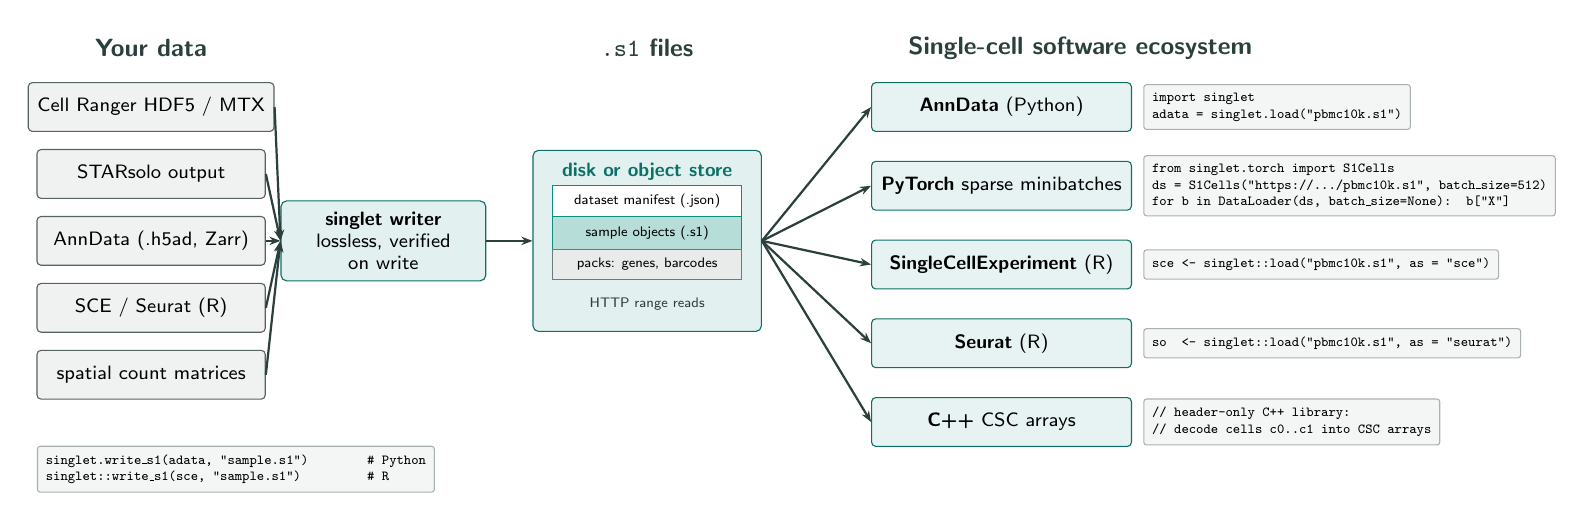
\begin{tikzpicture}[
  font=\sffamily\scriptsize,
  src/.style={draw=gen!80!black, fill=gen!10, rounded corners=1.5pt, minimum width=2.9cm, minimum height=0.62cm, align=center},
  hub/.style={draw=sone!80!black, fill=sone!12, rounded corners=2pt, align=center, inner sep=4pt},
  out/.style={draw=#1!80!black, fill=#1!10, rounded corners=1.5pt, minimum width=3.3cm, minimum height=0.62cm, align=center},
  code/.style={draw=ink2!40, fill=ink2!5, rounded corners=1pt, align=left, inner sep=3pt, font=\ttfamily\tiny, anchor=west},
  arr/.style={-{Stealth[length=4pt]}, thick, ink2},
  hdr/.style={font=\sffamily\small\bfseries, text=ink2},
]
% ---------- column headers ----------
\node[hdr] at (0,0.75) {Your data};
\node[hdr] at (6.3,0.75) {\sone{} files};
\node[hdr] at (11.8,0.75) {Single-cell software ecosystem};

% ---------- sources ----------
\node[src] (cr) at (0,0)     {Cell Ranger HDF5 / MTX};
\node[src] (ss) at (0,-0.85) {STARsolo output};
\node[src] (ad) at (0,-1.7)  {AnnData (.h5ad, Zarr)};
\node[src] (sr) at (0,-2.55) {SCE / Seurat (R)};
\node[src] (sp) at (0,-3.4)  {spatial count matrices};

% ---------- writer ----------
\node[hub, minimum width=2.6cm] (wr) at (2.95,-1.7) {\textbf{singlet writer}\\lossless, verified\\on write};
\foreach \s in {cr,ss,ad,sr,sp} \draw[arr] (\s.east) -- (wr.west);

% ---------- the objects ----------
\node[hub, minimum width=2.9cm, minimum height=2.3cm] (obj) at (6.3,-1.7) {};
\node[font=\sffamily\scriptsize\bfseries, text=sone!80!black] at (6.3,-0.82) {disk or object store};
\node[draw=sone, fill=white, minimum width=2.4cm, font=\sffamily\tiny] at (6.3,-1.2) {dataset manifest (.json)};
\node[draw=sone, fill=sone!30, minimum width=2.4cm, font=\sffamily\tiny] at (6.3,-1.6) {sample objects (.s1)};
\node[draw=gen, fill=gen!15, minimum width=2.4cm, font=\sffamily\tiny] at (6.3,-2.0) {packs: genes, barcodes};
\node[font=\sffamily\tiny, text=ink2] at (6.3,-2.5) {HTTP range reads};
\draw[arr] (wr.east) -- (obj.west);

% ---------- readers ----------
\node[out=sone] (py)  at (10.8,0.0)  {\textbf{AnnData} (Python)};
\node[out=sone] (pt)  at (10.8,-1.0) {\textbf{PyTorch} sparse minibatches};
\node[out=sone]   (sce) at (10.8,-2.0) {\textbf{SingleCellExperiment} (R)};
\node[out=sone]   (seu) at (10.8,-3.0) {\textbf{Seurat} (R)};
\node[out=sone]  (cpp) at (10.8,-4.0) {\textbf{C++} CSC arrays};
\foreach \o in {py,pt,sce,seu,cpp} \draw[arr] (obj.east) -- (\o.west);

% ---------- code beside each reader ----------
\node[code] at (12.6,0.0)  {import singlet\\adata = singlet.load("pbmc10k.s1")};
\node[code] at (12.6,-1.0) {from singlet.torch import S1Cells\\ds = S1Cells("https://.../pbmc10k.s1", batch\_size=512)\\for b in DataLoader(ds, batch\_size=None): b["X"]};
\node[code] at (12.6,-2.0) {sce <- singlet::load("pbmc10k.s1", as = "sce")};
\node[code] at (12.6,-3.0) {so \ <- singlet::load("pbmc10k.s1", as = "seurat")};
\node[code] at (12.6,-4.0) {// header-only C++ library:\\// decode cells c0..c1 into CSC arrays};

% ---------- writer calls ----------
\node[code] at (-1.45,-4.6) {singlet.write\_s1(adata, "sample.s1")\ \ \ \ \ \ \ \ \# Python\\singlet::write\_s1(sce, "sample.s1")\ \ \ \ \ \ \ \ \ \# R};
\end{tikzpicture}}
\caption{\textbf{\sone{} in the single-cell ecosystem.} Count matrices from Cell Ranger, STARsolo, AnnData,
SingleCellExperiment, Seurat or spatial pipelines are written once as \sone{} files, and the writer checks that the file
decodes to exactly the input. The \texttt{singlet} package reads them into AnnData, PyTorch minibatches,
SingleCellExperiment, Seurat or plain C++ arrays, from a local file or by HTTP range requests. The code beside each
target is the complete call (\texttt{DataLoader} is PyTorch's); Table~\ref{S-tab:eco} gives the time each takes on two
benchmark datasets. All calls are in \texttt{singlet}~\nm{rel-singlet_py} (Python) and \nm{rel-singlet_r} (R).}
\label{fig:eco}
\end{figure*}


% Discussion and conclusion (main text). Full limitations: Supplementary Limitations (supplement.tex).
\section{Discussion}
\label{sec:discussion}

Why have count matrices been stored so wastefully for so long? Generic arrays and byte compressors were a natural choice
while a matrix lived on the disk next to the analysis that used it. They fit poorly an archive of billions of cells read
across networks by models that see every cell many times. \sone{} instead describes the counts with what is known about
them, and the result sits close to every limit we could measure: within a few percent of the best count models we fitted
in size, on the trend of existing codes in decoding speed, and at the speed of a 1\,Gbit/s link on four cores.

In cloud storage, the bits per cell, the round trips per minibatch and the fees per request and per byte set both the speed
and the cost of every epoch. A format that is small, fast to decode and readable in part moves the bottleneck from storage
back to the model: a training loader started from a remote \sone{} file in under a second and kept the link busy without
downloading or converting anything first. The same latency matters even more to an AI agent working in a loop: an
agent that pulls the cells of one study, analyses them and decides what to fetch next waits on storage at every step, and a
second per fetch instead of a minute per download is the difference between iterating within one response and not
iterating at all. Because each sample file is named by a hash of its contents, a link or a citation identifies exactly the
bytes that were analysed, so an agent's analysis can be checked and repeated.

\para{Costs and limitations}\sone's decoder spends more time per entry than byte- or bit-aligned codes, so it keeps up with
a link only when there are enough cores for it: above about \nm{frac-cross-gbit}\,Gbit/s per decoding core, a larger but
faster code delivers more, and going faster at the same size would take a new kind of decoder, not a smaller file. Its
writer is slower than those of uncompressed formats and needs several times their memory. It stores whole-number counts
only, not the annotations of an AnnData object, so it complements rather than replaces such containers. And it is a format
for storing and moving counts, not for computing on them in place: unlike uncompressed HDF5 or Zarr arrays, its entries
cannot be memory-mapped and traversed without decoding. Because blocks decode independently and quickly, an out-of-core
analysis can instead stream a matrix block by block, holding only the cells it is working on. Our timings come from one
type of cluster node, and the network experiments from one emulated object store and one real one, read from one place
(Supplementary Limitations).

\para{Conclusion}\label{sec:conclusion}Count matrices are the one object that every single-cell analysis, and every model
trained on single-cell data, reads. \sone{} stores them close to their information content, decodes them as fast as the
trade-off between size and speed allows, reads them in part from anywhere, and returns exactly the original counts to
Python, R and C++. We propose it as a standard encoding for count matrices in archives, atlases and training pipelines,
and \texttt{pip install singlet} is all it takes to try it. The same structure, many small counts with heavy-tailed
frequencies, appears beyond single cells: bulk RNA-seq counts and a text corpus stored as word counts were also less than
half the size of compressed AnnData as \sone{} files (Supplementary Section~\ref{S-sec:beyond}).

% Methods (main text, after the Discussion): a summary. The full protocol is in the Supplementary Methods (supplement.tex).
\section{Methods}
\label{sec:setup}\label{sec:mmethods}

Every number, table and figure in this paper is produced by one pipeline from public data
(\texttt{papers/manuscripts/s1-format/bench} in the \texttt{singlet} repository); the Supplementary Methods
(Section~\ref{S-sec:methods}) give the full protocol, Supplementary Section~\ref{S-sec:sresults} the detailed results, and
Supplementary File~2 the format specification.

\para{Data}\nm{nMatrices} count matrices from \nm{nDatasets} public datasets in \nm{nProtocolClasses} protocol classes
(droplet, plate-based, combinatorial, multimodal and spatial data, from a thousand to more than a million cells;
Supplementary Table~\ref{S-tab:datasets}) were downloaded from their primary repositories, checked against recorded
SHA-256 digests and converted to one canonical sparse matrix with the source's gene identifiers and barcodes. Matrices with
non-integer values were rejected rather than rounded.

\para{Formats}Each format was written from the canonical matrix by its own library with default or recommended settings
(Supplementary Table~\ref{S-tab:formats}), read back and compared with the canonical matrix. File size includes gene
identifiers and barcodes.

\para{Read speed}Each read ran in a fresh process pinned to \nm{threadsHeadline} cores of a cluster node (\nm{cpu}), after
the library had been loaded and used once, untimed; files were evicted from the operating system's cache before each of
three timed repeats, and we report medians. The core sweep read the same files on 1 to 44 cores of an otherwise idle
48-core node.

\para{Training loaders}Loaders read minibatches of 512 cells, each made of eight blocks of 64 consecutive cells at random
offsets, into PyTorch sparse tensors, from a local S3-compatible object store whose bandwidth (0.1 to 10\,Gbit/s) and added
latency (0 to 200\,ms) we controlled, and from Cloudflare R2 over the public internet. We recorded the time from a new
process to the first minibatch and the time of each later one, for three seeds. Costs per epoch use the bytes and requests
counted at the emulated store and providers' published prices.

\para{Size floor}Poisson, negative binomial and nonparametric count models conditioned on cell depth, and on cell cluster,
were fitted on half of each matrix's cells and scored on the other half, zeros
included~\cite{hafemeister2019normalization,townes2019feature}. The shortest code length among them, charged nothing for
the models' own parameters, is our reference for the floor; it is a reference, not a bound.

\para{Speed frontier}A C++ benchmark (Supplementary Section~\ref{S-sec:mkernels}) encoded each matrix's row-index steps and values with raw 32-bit arrays, fixed-width
bytes, LEB128 varints, Stream VByte~\cite{lemire2018stream}, SIMD bit-packing~\cite{lemire2015decoding}, an order-0 rANS
coder~\cite{duda2013asymmetric}, and zstd at levels 3 and 19, and decoded each, and the \sone{} member, on one pinned core
(AVX2), checked against the input. Only writing the output arrays gives the rate no decoder can exceed by much; the
\emph{ideal code} stores the floor's code length and decodes at that rate. The trend is a power law, fitted to the other
codes' time per entry against their size on each matrix's frontier and evaluated at \sone's size, with an interval from
1,000 bootstrap resamples of the matrices.

\para{Write cost}Each format was written from the canonical matrix in memory, in a fresh process, recording wall time and
peak resident memory beyond the loaded input, each relative to writing uncompressed CSC arrays of the same matrix.


\section*{Data and code availability}
All datasets are public; accessions, file names, licenses and SHA-256 checksums are in \texttt{datasets.yaml} and
Supplementary Table~\ref{S-tab:datasets}. The \sone{} codec, its Python, R and C++ interfaces (\texttt{singlet}
\nm{rel-singlet_py} for Python and \nm{rel-singlet_r} for R, \url{https://github.com/Singlet-Bio/singlet}), and the
benchmark pipeline that produces every figure, table and number in this paper
(\texttt{papers/manuscripts/s1-format/bench}) are open source under the MIT license, with the per-stage results behind the
figures in \texttt{papers/manuscripts/s1-format/results}.

\section*{Acknowledgments}
Computations ran on the Clipper cluster at Grand Valley State University; the author thanks the GVSU HPC team for their
support. This work used Anvil at Purdue University through allocation BIO260157 from the Advanced Cyberinfrastructure
Coordination Ecosystem: Services \& Support (ACCESS) program, which is supported by U.S. National Science Foundation
grants \#2138259, \#2138286, \#2138307, \#2137603 and \#2138296. \emph{AI use:} Claude (Anthropic; Claude 5.5-generation models)~\cite{anthropicclaude} discovered the codec against benchmarks the author
designed, wrote all code and figures, and drafted the manuscript, its supplements and the author biography. The author designed the experiments
and evaluation, revised the text, verified all results, and is responsible for the content.

\bibliographystyle{IEEEtran}
\bibliography{refs}

\begin{IEEEbiographynophoto}{Zachary J. DeBruine}
received the Ph.D. degree from the Van Andel Institute Graduate School, Grand Rapids, MI, USA, in 2021, followed by
postdoctoral training at the Van Andel Institute. Since 2022 DeBruine has been an Assistant Professor in the College of
Computing at Grand Valley State University, Allendale, MI, USA, and an Adjunct Assistant Professor in the Department of
Epigenetics at the Van Andel Institute. DeBruine's research develops scalable methods and open data for single-cell
genomics, including fast non-negative matrix factorization (the RcppML package), compact sparse-matrix formats, and
singlet.bio, an open atlas of public single-cell RNA-seq data reprocessed from raw reads.
\end{IEEEbiographynophoto}

\end{document}
